\graphicspath{{5coset/asy/}}
\setcounter{section}{4}

\section{Cosets, Lagrange's Theorem \& Factor Groups}\label{chap:coset}

The overarching goal of this chapter is to partition a group into subsets in such a way that the \emph{set of subsets} inherits a natural group structure. This is a long and abstract story, though it is really nothing new; it is precisely the idea behind modular arithmetic!

\begin{example}{}{cosetsimple}
	In $\Z_3=\{0,1,2\}$ the elements are really \emph{subsets} $[0],[1],[2]$ of the \emph{integers} $\Z$: that is,
	\begin{gather*}
		[0]=\{x\in\Z:x \equiv 0\negthickspace\pmod 3\} =\{\ldots,-3,0,3,6,\ldots\}\\
		[1]=\{x\in\Z:x \equiv 1\negthickspace\pmod 3\} =\{\ldots,-2,1,4,7,\ldots\}\\
		[2]=\{x\in\Z:x \equiv 2\negthickspace\pmod 3\} =\{\ldots,-1,2,5,8,\ldots\}
	\end{gather*}
	When we write $1\operatorname{\textcolor{blue}{+_3}}2=0\in\Z_3$, what we really mean is
	\[
		\forall x\in[1], y\in[2]
		\text{ we have }
		x\operatorname{\textcolor{red}{+}}y\in [0]
	\]
	The \textcolor{red}{group operation (addition)} on $\Z$ naturally induces the \textcolor{blue}{group operation (addition modulo 3)} on the set of subsets $\Z_3=\{[0],[1],[2]\}$. 
\end{example}


\subsection{Cosets \& Normal Subgroups}\label{sec:cosetnormal}

Our primary goal is to generalize Example \ref{ex:cosetsimple}. Start by observing that the identity element $[0]\in\Z_3$ is a \emph{subgroup} of $\Z$ from which the other subsets $[1]$, $[2]$ may be obtained by \emph{translation.}

\begin{defn}{}{}
	Let $H$ be a subgroup of $G$ and $g\in G$. The \emph{left coset} of $H$ containing $g$ is 
	\[
		gH:=\{gh:h\in H\}\tag{$x\in gH\iff \exists h\in H$ such that $x=gh$}
	\]
	This is a subset of $G$. The \emph{right coset} of $H$ containing $g$ is defined similarly:
	\[
		Hg:=\{hg:h\in H\}
	\]
	The \emph{identity coset} $H=eH=He$ is the left \& right coset of $H$ containing the identity $e$.\smallbreak
	$H$ is a \emph{normal subgroup} of $G$, written $H\triangleleft G$, if the left and right cosets containing $g$ are always equal
	\[
		H\triangleleft G
		\iff
		\forall g\in G,\ gH=Hg
	\]
\end{defn}

If $G$ is written additively, then the left and right cosets of $H$ containing $g$ are instead written
\[
	g+H:=\{g+h:h\in H\}
	\qquad\qquad 
	H+g:=\{h+g:h\in H\}
\]

\begin{example*}{\ref{ex:cosetsimple} cont}{}
	Let $G=\Z$ and $H=[0]=3\Z$. The left and right cosets of $H$ are precisely the elements of $\Z_3$:
	\begin{gather*}
		3\Z=0+3\Z=3\Z+0=[0]=\{\ldots,-3,0,3,6,\ldots\}\\
		1+3\Z=3\Z+1=[1]=\{\ldots,-2,1,4,7,\ldots\}\\
		2+3\Z=3\Z+2=[2]=\{\ldots,-1,2,5,8,\ldots\}
	\end{gather*}
	Since the left and right cosets are equal, $H=3\Z$ is a normal subgroup of $\Z$.
\end{example*}

\goodbreak

The last observation is in fact general---the proof is an exercise.

\begin{lemm}{}{cosetbasic1}
	Every subgroup of an abelian group $G$ is normal.
\end{lemm}


A subgroup of a non-abelian group \emph{might} be normal, but is more likely not to be (see Example \ref*{ex:cosetexs}.\ref{ex:nonnormalcosets}).


\begin{examples}{}{cosetexs}
	\exstart\label{ex:cosets1} The subgroup $H=\ip 2=\{0,2,4\}\le\Z_6$ has two distinct cosets (left $=$ right since $\Z_6$ is abelian):
	\begin{align*}
		H&=\{0,2,4\}&&\bigl(=2+H=4+H\bigr)\\
		1+H&=\{1,3,5\}&&\bigl(=3+H=5+H\bigr)
	\end{align*}
	Observe how the cosets \textbf{partition} $\Z_6$ into equal-sized subsets.
	
% 	\exstart\label{ex:cosets1} Consider the subgroup $H=\ip 4=\{0,4,8\}\le\Z_{12}$. This is cyclic with order 3. The distinct cosets of $\ip 4$ are as follows (left $=$ right since $\Z_{12}$ is abelian!):
% 	\begin{align*}
% 		\ip 4 &=\{0,4,8\}&&\bigl(=4+\ip 4=8+\ip 4\bigr) \hspace{220pt}\\
% 		1+\ip 4 &=\{1,5,9\}&&\bigl(=5+\ip 4=9+\ip 4\bigr)\\
% 		2+\ip 4 &=\{2,6,10\}&&\bigl(=6+\ip 4=10+\ip 4\bigr)\\
% 		3+\ip 4 &=\{3,7,11\}&&\bigl(=7+\ip 4=11+\ip 4\bigr)
% 	\end{align*}
% 	Observe how the cosets \emph{partition} $\Z_{12}$ into equal-sized subsets. 

	\begin{enumerate}\setcounter{enumi}{1}
		\item\label{ex:nonnormalcosets} The left and right cosets of the subgroup $H=\{e,\mu_1\}\le D_3$ are as follows:
		\[
			\renewcommand{\arraystretch}{1.15}
			\begin{array}{l@{\hspace*{.3cm}}|@{\hspace*{.3cm}}l}
		  	\text{Left cosets} & \text{Right cosets}\\\hline
				H=\mu_1H=\{e,\mu_1\}& H=H\mu_1=\{e,\mu_1\}\\
				\rho_1H=\mu_3H=\{\rho_1,\mu_3\} & H\rho_1=H\mu_2=\{\rho_1,\mu_2\}\\
				\rho_2H=\mu_2H=\{\rho_2,\mu_2\} & H\rho_2=H\mu_3=\{\rho_1,\mu_3\}
			\end{array}
		\]
		To verify this, either revisit the multiplication table for $D_3$ (Example \ref{ex:d3}) or use cycle notation (e.g. Example \ref{ex:disym}).	This time the left and right cosets of $H$ are not the same: $H$ is \emph{not} a normal subgroup of $D_3$. The \textbf{partitioning} observation still holds: the left cosets partition $D_3$ into three equal-sized subsets; the right cosets also partition $D_3$ into equal-sized (but different) subsets.
	
	  
		\begin{minipage}[t]{0.65\linewidth}\vspace{0pt}
			\item\label{ex:cosetsubspace} Consider a 1-dimensional subspace $\textcolor{blue}{W}\le\R^2$. Each coset
			\[
				\textcolor{Green}{\vu+W} =\{\vu+\vw:\vw\in W\}
			\]
			is a line parallel to $W$. Once again, the cosets (all lines parallel to $W$) \textbf{partition} $\R^2$.\smallbreak
			If this feels too abstract, consider the special case where $W$ is the $y$-axis: each coset is a vertical line (same $x$-co-ordinate).\smallbreak
			More generally, if $W$ is a subspace of some vector space, then the cosets $\vu+W$ are the sets parallel to $W$. Only the zero coset $W=\V0+W$ is a sub\emph{space.}
		\end{minipage}
		\hfill
		\begin{minipage}[t]{0.33\linewidth}\vspace{0pt}
			\flushright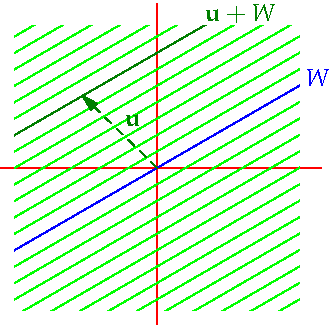
\includegraphics[scale=0.93]{coset-coset}
		\end{minipage}
	
	
		\item Consider the alternating group $A_n$ as a subgroup of $S_n$. Generalizing the argument from Theorem \ref{thm:alt}, we see that for any $\alpha\in A_n$ and $\sigma\in S_n$,
		\[
			\alpha\sigma\text{ even }
			\iff \sigma\text{ even }
			\iff \sigma\alpha\text{ even}
		\]
		Otherwise said, for any $\sigma\in S_n$ the cosets of $A_n$ containing $\sigma$ are
		\[
			\sigma A_n=A_n\sigma=
			\begin{cases}
				A_n&\text{if $\sigma$ even}\\
				B_n&\text{if $\sigma$ odd}
			\end{cases}
		\]
		where $B_n$ is the set of odd permutations in $S_n$. In particular, $A_n$ is a normal subgroup of $S_n$.
	\end{enumerate}
\end{examples}


\goodbreak


As observed in the examples, the cosets of any subgroup $H\le G$ partition $G$.

\begin{thm}{}{cosetpart}
	Let $H$ be a subgroup of $G$. Then the left cosets of $H$ partition $G$. Moreover,
	\[
		y\in xH
		\mathrel{\textcolor{blue}{\iff}} x^{-1}y\in H
		\mathrel{\textcolor{red}{\iff}} xH=yH
	\]
	The right cosets also partition $G$:
	\[
		y\in Hx\iff yx^{-1}\in H\iff Hx=Hy
	\]
\end{thm}

The \textcolor{blue}{blue} criterion is often very easy to check. Before reading the proof, convince yourself that each of our previous examples satisfies the result. When $H$ is non-normal, the right cosets partition $G$ differently to the left cosets (e.g.\ Example \ref*{ex:cosetexs}.\ref{ex:nonnormalcosets}).

\begin{example}{}{}
	This should seem familiar when $G=\Z$ and $H=n\Z$. Written additively,
	\[
		a+H=b+H\mathrel{\textcolor{red}{\iff}} b-a\in H\iff n\mid b-a \iff a\equiv b\pmod n
	\]
	The cosets of $H$ are precisely the equivalence classes modulo $n$. Indeed you've likely encountered the main proof in the context of modular arithmetic.
\end{example}

\begin{proof}
	We start by verifying the \textcolor{blue}{first connective}.
	\[
		y\in xH
		\iff \exists h\in H\text{ such that }y=xh
		\iff x^{-1}y=h\in H
	\]
	Now define a relation $\sim$ on $G$ via $x\sim y\Longleftrightarrow x^{-1}y\in H$. We claim that this is an equivalence relation:
	\begin{quote}
		\begin{description}\itemsep2pt
			\item[\normalfont\emph{Reflexivity}:] $x\sim x$ since $x^{-1}x=\textcolor{Green}{e\in H}$.
			\item[\normalfont\emph{Symmetry}:] $x\sim y\Longrightarrow x^{-1}y\in H \mathrel{\textcolor{Green}{\Longrightarrow}} y^{-1}x=(x^{-1}y)^{-1}\in H \Longrightarrow y\sim x$.
			\item[\normalfont\emph{Transitivity}:] If $x\sim y$ and $y\sim z$ then $x^{-1}y\in H$ and $y^{-1}z\in H$. But \textcolor{Green}{$H$ is closed}, whence
			\[
				x^{-1}z=(x^{-1}y)(y^{-1}z)\in H\implies x\sim z
			\]
		\end{description}
	\end{quote}
	The equivalence classes therefore partition $G$. Since $x\sim y\iff y\in xH$, the equivalence class of $x$ is indeed the left coset $xH$.\qedhere
\end{proof}



The \textcolor{Green}{subgroup status} of $H$ is precisely what guarantees a partition (compare Theorem \ref{thm:subgroup}):
\begin{quote}
	\begin{description}\itemsep2pt
		\item[\normalfont\emph{Reflexivity}:]  $H$ contains the \textcolor{Green}{identity} (and is thus \textcolor{Green}{non-empty}).
		\item[\normalfont\emph{Symmetry}:] $H$ satisfies the \textcolor{Green}{inverse axiom}.
		\item[\normalfont\emph{Transitivity}:] $H$ is \textcolor{Green}{closed} under the group operation.
	\end{description}
\end{quote}

When $H$ is not a subgroup, the coset construction need not produce a partition.

\begin{example}{}{}
	The \emph{subset} $H=\{0,1\}\subseteq\Z_3$ is not a subgroup. Its left `cosets' fail to partition $\Z_3$:
	\[
		H=\{0,1\},\quad 1+H=\{1,2\},\quad 2+H=\{2,1\}
	\]
\end{example}


\goodbreak

By combining the criteria in Theorem \ref{thm:cosetpart}, we obtain a useful result for identifying when a subgroup is normal \emph{without} explicitly having to compute its cosets. The proof is an exercise.

\begin{cor}{}{normalconj}
	Normal subgroups are precisely those which are closed under \textbf{conjugation}:
  \[
  	H\triangleleft G\iff H\le G\text{ and \ }\forall g\in G,\ \forall h\in H, \	gh g^{-1}\in H
  \]
\end{cor}

Since this holds for all $g$, we may equivalently observe $g^{-1}hg\in H$. 

% \begin{proof}
% 	Start by using the criteria in Theorem \ref{thm:cosetpart} to observe:
% 	\begin{enumeratea}
% 	  \item $gH\subseteq Hg\iff \forall h\in H,\ gh\in Hg \iff \forall h\in H,\ gh g^{-1}\in H$
% 	  \item $Hg\subseteq gH\iff \forall h\in H,\ hg\in gH \iff \forall h\in H,\ g^{-1}hg\in H$
% 	\end{enumeratea}
% 	We now complete the proof in two parts:
% 	\begin{description}
% 		\item[\normalfont $(\Rightarrow)$] $H\triangleleft G$ means $\forall g\in G,\ Hg=gH$, and so implies part (a) for all $g\in G$. 
% 		\item[\normalfont $(\Leftarrow)$] If $gh g^{-1}\in H$ for all $g,h$, then this is also true for $g^{-1}$: that is $g^{-1}hg\in H$. We now have the right side of both (a) and (b). Otherwise said, $gH=Hg$ for all $g\in G$, whence $H$ is normal in $G$.\qedhere
% 	\end{description}
% \end{proof}


\boldsubsubsection{Kernels and Normal Subgroups}

In Exercise \ref*{sec:morph}.\ref{exs:kernelintro} we defined the \emph{kernel} and \emph{image} of a homomorphism $\phi:G\to L$:
\[
	\ker\phi =\bigl\{g\in G:\phi(g)=e\bigr\},\qquad \image\phi=\bigl\{\phi(g):g\in G\bigr\}
\]
and verified that these are \emph{subgroups} (of $G$ and $L$ respectively). The rest of this section describes part of the intimate relationship between kernels, images and normal subgroups; a relationship that will be explained more fully in Section \ref{sec:1stiso}.


\begin{examples}{}{}
	\exstart It is easily checked that $\phi(x)=2x\pmod 4$ defines a homomorphism $\phi:\Z\to\Z_4$. We compute:
	\[
		\ker\phi=\{x\in\Z:2x\equiv 0\negthickspace\pmod 4\}=2\Z,
		\qquad
		\image\phi=\{0,2\}
	\]
	Plainly $\ker\phi$ is a subgroup of $\Z$ and $\image\phi$ is a subgroup of $\Z_4$.
	\begin{enumerate}\setcounter{enumi}{1}
	  \item Every linear map $\rT:V\to W$ between vector spaces is a homomorphism. In linear algebra its kernel is better known as its \emph{nullspace}
		\[
			\ker\rT=\mathcal N(\rT)=\bigl\{\vv\in V:\rT(\vv)=\V0\bigr\}
		\]
		If $\rT=\rL_A:\R^n\to \R^m$ is left-multiplication by a matrix $A$, then $\image\rT$ is the \emph{column space} of $A$.
	\end{enumerate}
\end{examples}

Since the groups in these examples are all abelian, all subgroups are automatically normal. In fact the kernel of \emph{every} homomorphism is a normal subgroup, though the same cannot be said for images.

\begin{lemm}{}{homosub}
	If $\phi:G\to L$ is a homomorphism, then $\ker\phi\triangleleft G$.
\end{lemm}

\begin{proof}
	Exercise \ref*{sec:morph}.\ref{exs:structural1} verified that $\ker\phi\le G$. For normality, we appeal to Corollary \ref{cor:normalconj}. Let $g\in G$, $k\in\ker\phi$, apply the homomorphism property and the fact that $\phi(g^{-1})=\phi(g)^{-1}$ (Exercise \ref{sec:morph}.\ref{exs:structural2}):
	\[
		\phi(gk g^{-1})=\phi(g)\phi(k)\phi(g)^{-1}
	  =\phi(g)\phi(g)^{-1}=e_L
	  \implies gk g^{-1}\in\ker\phi\tag*{\qedhere}
	\]
\end{proof}


\begin{examples}{}{}
	\exstart $\det:\rGL_n(\R)\to\R^\times$ is a homomorphism. We obtain a normal subgroup
	\[
		\ker\det=\{A\in\rGL_n(\R):\det A=1\}
		\triangleleft\rGL_n(\R)
	\]
	Otherwise said, $\rSL_n(\R)$ is a normal subgroup of $\rGL_n(\R)$.
	\begin{enumerate}\setcounter{enumi}{1}
  	\item (Example \ref*{ex:cosetexs}.\ref{ex:nonnormalcosets}, cont.) \ $\phi:\Z_2\to D_3$ defined by $\phi(x)=\mu_1^x$ is a homomorphism. Certainly $\ker\phi=\{0\}\triangleleft\Z_2$, however $\image\phi=\{e,\mu_1\}$ is not a \emph{normal} subgroup of $S_3$.
	\end{enumerate}
\end{examples}

\goodbreak


\begin{exercises}{}{}
	Key concepts:\quad \emph{left/right cosets \& partitioning\quad normal subgroup\quad kernels are normal}

	\begin{enumerate}
	  \item Find the cosets of each subgroup: since the groups are abelian, left and right cosets are equal.
		\begin{enumerate}
	  	\item $2\Z\le\Z$\qquad\quad
	  	(b) $4\Z\le 2\Z$\qquad\quad
		  (c) $\ip{4}\le\Z_{10}$\qquad\quad
		  (d) $\ip{6}\le\Z_{30}$\qquad\quad
		  (e) $\ip{20}\le\Z_{30}$
		\end{enumerate}
			
			
		\item\label{exs:VfactorV} Find the cosets of $H=\bigl\{(0,0),(2,0),(0,2),(2,2)\bigr\}\le\Z_4\times\Z_4$
			
			
		\item Find the left and right cosets of $\{\rho_0,\rho_1,\rho_2\}\le D_3$. Is the subgroup normal?
		
		
		\item\label{exs:va4}\begin{enumerate}
		  \item Find the left and right cosets of $H:=\{e,(1\,2\,3),(1\,3\,2)\}\le A_4$. Is the subgroup normal?
		  \item Repeat the question for the subgroup $V:=\{e,(1\,2)(3\,4),(1\,3)(2\,4),(1\,4)(2\,3)\}$
		\end{enumerate}
		
	
		\item\label{exs:d4normal}\begin{enumerate}
		  \item Find the left and right cosets of $H=\{\rho_0,\delta_1\}\le D_4$. Is $H$ normal? (see Examples \ref{ex:disym})
			\item Repeat for the subgroup $K=\{\rho_0,\rho_2\}$.
		\end{enumerate}
	  
	  
	  \item Prove Lemma \ref{lemm:cosetbasic1}: every subgroup of an abelian group is normal.
	  
	  
	  \item\label{exs:partitioncoset} Suppose $H$ is a \emph{subset} of $G$, but not necessarily a subgroup.
	  \begin{enumerate}
	    \item If $H$ has only one element, show that the sets $gH=\{gh:h\in H\}$ do partition $G$.
	    \item Show that the `cosets' of $H=\{1,3\}$ also partition $\Z_4$, even though $H$ is not a subgroup.
	  \end{enumerate}
	  
	
		\item Let $H=\{\sigma\in S_4:\sigma(4)=4\}$. Show that $H$ is a subgroup of $S_4$. Is it \emph{normal}?
		
		
		\item Prove Corollary \ref{cor:normalconj}.
	  
	  
	  \item\label{exs:directprodfactor}\begin{enumerate}
	    \item Suppose $G=H\times K$, \ $J\triangleleft H$ and let $\widetilde J=J\times\{e_K\}$. Prove that $\widetilde J\triangleleft G$.\par
	    (\emph{When $J=H$ this is often written $H\triangleleft (H\times K)$. A similar result holds for $K$.})
	    \item Explain how Example \ref*{ex:cosetexs}.\ref{ex:cosetsubspace} fits into part (a).
	  \end{enumerate} 
	  
		
		\item Let $H,K$ be subgroups of $G$. Define $\sim$ on $G$ by
		\[
			a\sim b\iff \exists h\in H,\ k\in K \ \text{ such that }\ a=hb k
		\]
		\begin{enumerate}
	  	\item Prove that $\sim$ is an equivalence relation on $G$ and describe the elements of the equivalence class of $a\in G$; this is called a \emph{double coset}.
	  	\item Compute the double cosets of $H=\{e,(1\,2)\}$ and $K=\{e,(1\,3)\}$ as subgroups of $S_3$. 
		\end{enumerate}
		
		
		\item Verify that $\phi:\Z\to\Z_n:x\mapsto x\pmod n$ is a homomorphism. What is its kernel? 
			
		\item State a linear map $\rT:\R^2\to\R^2$ whose kernel is the $y$-axis (a normal subgroup of $\R^2$\ldots)
		
		
		\item Find the kernel and image of each homomorphism and verify that $\ker\phi$ is normal:
		\begin{enumerate}
		  \item The \emph{trace} of a matrix $\tr:M_2(\R)\to\R:
		  \smash{
			  \begin{smatrix}
					a&b\\c&d
			  \end{smatrix}
		  }
		  \mapsto a+d$.
			
			\item $\rT:\R^3\to\R^4:\vx\mapsto 
			\begin{smatrix}
				1&1&-1\\
				0&3&-1\\
				1&4&-2\\
				2&5&-3
			\end{smatrix}$
		\end{enumerate}
		
		
		\item Explain why the map $\phi$ is a homomorphism and find $\ker\phi$:
		\[
			\phi:S_n\to \bigl(\{1,-1\},\cdot\bigr):\sigma \mapsto 
			\begin{cases}
	  		1&\text{ if $\sigma$ even}\\
	  		-1&\text{ if $\sigma$ odd}
			\end{cases}
		\]
		
		
	  \item Consider $\phi:D_4\to D_4:\sigma\mapsto \sigma^2$. Show that $\phi$ is \emph{not} a homomorphism.
	\end{enumerate}
\end{exercises}


\clearpage


\subsection{Lagrange's Theorem \& Indices (Counting Cosets)}\label{sec:lagrange}


We've been inching towards a powerful result; hopefully you've hypothesized this already!

\begin{thm}{Lagrange}{lagrange}
	In a finite group, the order of a subgroup divides the order of the group:\footnotemark
	\[
		H\le G\implies \nm H\Big\vert \nm G
	\]
\end{thm}

Note that the converse is \emph{false}: e.g.{} $A_4$ has order 12, but no subgroup of order 6 (Exercise \ref*{sec:transpositions}.\ref{exs:a4subgroups}). The argument is merely a generalized version of the proof of Theorem \ref{thm:alt} ($\nm{A_n}=\frac 12\nm{S_n}$).

\footnotetext{%
	This is often misremembered as `the order of an element divides the order of the group,' which is the special case when $H$ is a \emph{cyclic subgroup} of $G$. Corollary \ref{cor:subscyclic} is the even more special case when $G$ is cyclic:
	$\ip s\le\Z_n$ has order $\frac n{\gcd(s,n)}$.
}


\begin{proof}
	Suppose $H\le G$ and fix $g\in G$. The function \emph{left-multiplication by $g$}
	\[
		L_g:H\to gH:h\mapsto gh
	\]
	is a bijection (with inverse $L_g^{-1}:gh\mapsto h$). Every left coset of $H$ therefore has the same cardinality as $H$. Since the left cosets partition $G$ (Theorem \ref{thm:cosetpart}), we conclude that
	\[
		\nm G=\text{(number of left cosets of $H$)}\cdot \nm H
		\implies \nm H\Big\vert \nm G
		\tag*{\qedhere}
	\]
\end{proof}


We could instead have proved Lagrange via the right coset partition. Here is an example of its power.

\begin{cor}{}{}
	Up to isomorphism, there is a unique group of prime order $p$, namely $\Z_p$.
\end{cor}

\begin{proof}
	Suppose $G$ is a group with prime order $p$. Since $p\ge 2$, we may choose some element $g\neq e$. The order of the cyclic subgroup $\ip{g}\le G$ satisfies:
	\begin{itemize}%\itemsep0pt
	  \item $\nm{\ip g}\ge 2$ since $g\neq e$.
	  \item $\nm{\ip{g}}=1$ or $p$ by Lagrange, since $p$ is prime.
	\end{itemize}
	We conclude that $\nm{\ip g}=p\implies G=\ip{g}$ is cyclic and thus isomorphic to $\Z_p$ (Theorem \ref{thm:cyclicisomorph}).
\end{proof}

\begin{example}{}{}
	$G=\Z_4\times\Z_2$ has order 8 so its non-trivial proper subgroups can only have orders 2 or 4 and are thus isomorphic to $\Z_2$, $\Z_4$ or $\textcolor{blue}{V}$. These can be identified by thinking about all possible generators; $V$ requires three elements of order 2 which we indeed have! Here is the subgroup diagram: all proper subgroups are cyclic except \textcolor{blue}{$V=\{(0,0),(2,0),(0,1),(2,1)\}$}.
	\[
		\def\arraystretch{1.1}
		\begin{array}[t]{@{}c|c|c}
			\text{generator}&\text{order}&\text{subgroup}\\\hline
			(1,0)\text{ or }(3,0) & 4 & \{(0,0),(1,0),(2,0),(3,0)\}\\
			(1,1)\text{ or }(3,1) & 4 & \{(0,0),(1,1),(2,0),(3,1)\}\\
			(2,0) & 2 & \{(0,0),(2,0)\}\\
			(0,1) & 2 & \{(0,0),(0,1)\}\\
			(2,1) & 2 & \{(0,0),(2,1)\}\\
			(0,0) & 1 & \{(0,0)\}
		\end{array}
		\qquad
		\xymatrix @R13pt{%
			&\Z_4\times\Z_2 \ar@/_0pc/@{-}[dl] \ar@{-}[d] \ar@{-}[dr]&\\
			\ip{(1,0)} \ar@{-}[dr] & \textcolor{blue}{V} \ar@{-}[dl] \ar@{-}[d] \ar@{-}[dr] & \ip{(1,1)} \ar@{-}[dl]\\
			\ip{(0,1)} \ar@{-}[dr] & \ip{(2,0)} \ar@{-}[d] & \ip{(2,1)} \ar@{-}[dl] &\\
			&\ip{(0,0)}&
		}
	\]
\end{example}


\goodbreak


The proof of Lagrange tells us that the \emph{number} of left and right cosets of $H\le G$ is \emph{identical:} both equal the quotient $\frac{\nm G}{\nm H}$. This motivates a new concept.

\begin{defn}{}{index}
	The \emph{index} $(G:H)$ of a subgroup $H\le G$ is the cardinality of the set of (left) cosets:
	\[
		(G:H)=\nm{\{gH:g\in G\}}
	\]
\end{defn}

The index is also the cardinality of the set of \emph{right} cosets (Exercise \ref{exs:indexcard}). If $G$ is finite, then $(G:H)=\frac{\nm G}{\nm H}$.


\begin{examples}{}{indexeasy}
	\exstart If $G=\Z_{20}$ and $H=\ip{2}$, then there are $(G:H)=\frac{20}{10}=\frac{\nm G}{\nm H}=2$ cosets:
	\[
		H=\ip{2}=\{0,2,4,\ldots,18\}
		\quad\text{and}\quad 
		1+H=\{1,3,5,\ldots,19\}
		\]
	\begin{enumerate}\setcounter{enumi}{1}
	  \item\label{ex:indexeasy2} Recall (Example \ref{ex:orthogonal} \& Exercise \ref*{sec:subgroup}.\ref{exs:subgpmatrix}) the orthogonal and special orthogonal groups
	  \[
	  	\rO_n(\R)=\{A\in M_n(\R):A^TA=I\},\qquad
	  	\rSO_n(\R)=\{A\in\rO_n(\R):\det A=1\}
	  \]
	  Since every orthogonal matrix has determinant $\pm 1$, it feels as if $\rSO_n(\R)$ should be `half' of $\rO_2(\R)$. Since both groups are infinite (indeed uncountable), we need the index to confirm this intuition. Recall Theorem \ref{thm:cosetpart}: given $A,B\in\rO_n(\R)$,
	  \[
	  	A\,\rSO_n=B\,\rSO_n(\R)
	  	\iff B^{-1}A\in\rSO_n(\R)
	  	\iff \det(B^{-1}A)=1
	  	\iff \det B=\det A
	  \]
	  We conclude that there are precisely two cosets $\bigl(\rO_n(\R):\rSO_n(\R)\bigr)=2$.
	\end{enumerate}
\end{examples}


\begin{thm}{}{tower}
	If $K\le H\le G$ is a sequence of subgroups, then
	\[
		(G:K)=(G:H)(H:K)
	\]
\end{thm}

If $G$ is a finite group then the result is essentially trivial:
\[
	(G:K)=\frac{\nm G}{\nm K}
	=\frac{\nm G}{\nm H}\cdot\frac{\nm H}{\nm K}
	=(G:H)(H:K)
\]
Our proof also covers infinite groups and infinite indices. You are \emph{strongly} encouraged to work through the following examples, which are written in the language of the proof.



\begin{proof}
	Choose an element $\textcolor{red}{g_i}$ from each left coset of $H$ in $G$ and an element $\textcolor{blue}{h_j}$ from each left coset of $K$ in $H$. Plainly
	\[
		(G:H)=\nm{\{\textcolor{red}{g_i}\}}
		\qquad\text{and}\qquad 
		(H:K)=\nm{\{\textcolor{blue}{h_j}\}}
	\]
	We claim that the left cosets of $K$ in $G$ are precisely the sets $(\textcolor{red}{g_i}\textcolor{blue}{h_j})K$. Certainly each such is a \emph{coset}; we show that these cosets \emph{partition} $G$, whence the collection $\{(\textcolor{red}{g_i}\textcolor{blue}{h_j})K\}$ must comprise \emph{all} left cosets.
	\begin{itemize}
	  \item Every $g\in G$ lies in some left coset of $H$, so $\exists \textcolor{red}{g_i}\in G$ such that $g\in \textcolor{red}{g_i}H$.\par
	  $\textcolor{red}{g_i}^{-1}g\in H$ lies in some left coset of $K$ in $H$, so $\exists \textcolor{blue}{h_j}\in H$ such that $\textcolor{red}{g_i}^{-1}g\in \textcolor{blue}{h_j}K$.\par
	  But then $g\in (\textcolor{red}{g_i}\textcolor{blue}{h_j})K$ so that every $g\in G$ lies in at least one set $(\textcolor{red}{g_i}\textcolor{blue}{h_j})K$.
	  \item Suppose $y\in \textcolor{red}{g_i}\textcolor{blue}{h_j}K\cap \textcolor{red}{g_\alpha} \textcolor{blue}{h_\beta}K$. Since $K\le H$ and the left cosets of $H$ partition $G$, we have
	  \[
	  	y\in \textcolor{red}{g_i}H\cap \textcolor{red}{g_\alpha} H
	  	\implies \textcolor{red}{g_\alpha}=\textcolor{red}{g_i}
	  \]
	  But then $\textcolor{red}{g_i}^{-1}y\in \textcolor{blue}{h_j}K\cap \textcolor{blue}{h_\beta} K\implies \textcolor{blue}{h_\beta}=\textcolor{blue}{h_j}$ similarly, since the left cosets of $K$ in $H$ partition $H$. It follows that the sets $(\textcolor{red}{g_i}\textcolor{blue}{h_j})K$ are disjoint.
	\end{itemize}
	Since the left cosets of $K$ in $G$ are given by $\{(g_i\textcolor{blue}{h_j})K\}$, it is immediate that
	\[
		(G:K)=\nm{\{g_i\textcolor{blue}{h_j}\}}
		=\nm{\{g_i\}}\nm{\{\textcolor{blue}{h_j}\}}
		=(G:H)(H:K)
		\tag*{\qedhere}
	\]
\end{proof}



\begin{examples}{}{}
	\exstart Recall Example \ref{ex:indexeasy}.1: let $G=\Z_{20}$, $H=\ip{2}$ and $K=\ip{10}$. Plainly
	\[
		K=\{0,10\}
		\le H=\{0,2,4,6,8,10,12,14,16,18\}
		\le G=\{0,1,2,3,\ldots,19\}
	\]
	so we have the required subgroup relationship. Here are the indices and cosets in each case:
		
	\begin{enumerate}\setcounter{enumi}{1}
	  \item[]\begin{itemize}
		  \item $(G:H)=2$ with cosets $H$ and $\textcolor{red}{1}+H$. In the language of the proof, $\textcolor{red}{g_0=0}$ and $\textcolor{red}{g_1=1}$.
		  \item $(H:K)=\frac{10}{2}=5$ cosets, with representatives $\textcolor{blue}{h_0=0}$, $\textcolor{blue}{h_1=2}$, $\textcolor{blue}{h_2=4}$, $\textcolor{blue}{h_3=6}$, $\textcolor{blue}{h_4=8}$:
			\[
				K=\{0,10\},\ \ \textcolor{blue}{2}+K=\{2,12\},\ \ \textcolor{blue}{4}+K=\{4,14\},\ \ \textcolor{blue}{6}+K=\{6,16\},\ \ \textcolor{blue}{8}+K=\{8,18\}
			\]
			\item $(G:K)=\frac{20}{2}=10=(G:H)(H:K)$: the cosets are
			\[
				K=\{0,10\},\quad 
				1+K=\{1,11\},\quad 
				2+K=\{2,12\},\quad 
				\ldots ,\quad 
				9+K=\{9,19\}
			\]
			In the language of the proof these cosets all have the form $(\textcolor{red}{g_i}+\textcolor{blue}{h_j})+K$.
		\end{itemize}
	
		\item Consider the sequence of subgroups $K\le H\le S_4$ where
		\[
			K=\{e,(1\,2\,3),(1\,3\,2)\}\cong\Z_3
			\quad\text{and}\quad 
			H=\{\sigma\in S_4:\sigma(4)=4\}\cong S_3
		\]
		The $(H:K)=\frac 63=2$ left cosets of $K$ in $H$ are
		\[
			K=\textcolor{blue}{e}K=\{e,(1\,2\,3),(1\,3\,2)\}
			\quad\text{and}\quad 
			\textcolor{blue}{(1\,2)}K=\{(1\,2),(2\,3),(1\,3)\}
		\]
		with representatives $\textcolor{blue}{h_0=e}$ and $\textcolor{blue}{h_1=(1\,2)}$. The $(S_4:H)=\frac{24}6=4$ left cosets of $H$ in $S_4$ are
		\begin{gather*}
			H=\textcolor{red}{e}H=\{e,(1\,2\,3),(1\,3\,2),(1\,2),(2\,3),(1\,3)\}\\
			\textcolor{red}{(1\,4)}H=\{(1\,4),(1\,2\,3\,4),(1\,3\,2\,4),(1\,2\,4),(1\,4)(2\,3),(1\,3\,4)\}\\
			\textcolor{red}{(2\,4)}H=\{(2\,4),(1\,4\,2\,3),(1\,3\,4\,2),(1\,4\,2),(2\,3\,4),(1\,3)(2\,4)\}\\
			\textcolor{red}{(3\,4)}H=\{(3\,4),(1\,2\,4\,3),(1\,4\,3\,2),(1\,2)(3\,4),(2\,4\,3),(1\,4\,3)\}
		\end{gather*}
		with representatives $\textcolor{red}{g_0=e}$, $\textcolor{red}{g_1=(1\,4)}$, $\textcolor{red}{g_2=(2\,4)}$, $\textcolor{red}{g_3=(3\,4)}$. The \emph{eight} left cosets of $K$ in $S_4$ are therefore
		\begin{align*}
			&\textcolor{red}{e}\textcolor{blue}{e}K=K=\{e,(1\,2\,3),(1\,3\,2)\}&&\textcolor{red}{e}\textcolor{blue}{(1\,2)}K=\textcolor{blue}{(1\,2)}K=\{(1\,2),(2\,3),(1\,3)\}\\
			&\textcolor{red}{(1\,4)}\textcolor{blue}{e}K=\textcolor{red}{(1\,4)}K=\{(1\,4),(1\,2\,3\,4),(1\,3\,2\,4)\}&&\textcolor{red}{(1\,4)}\textcolor{blue}{(1\,2)}K=\{(1\,2\,4),(1\,4)(2\,3),(1\,3\,4)\}\\
			&\textcolor{red}{(2\,4)}\textcolor{blue}{e}K=\textcolor{red}{(2\,4)}K=\{(2\,4),(1\,4\,2\,3),(1\,3\,4\,2)\}&&\textcolor{red}{(2\,4)}\textcolor{blue}{(1\,2)}K=\{(1\,4\,2),(2\,3\,4),(1\,3)(2\,4)\}\\
			&\textcolor{red}{(3\,4)}\textcolor{blue}{e}K=\textcolor{red}{(3\,4)}K=\{(3\,4),(1\,2\,4\,3),(1\,4\,3\,2)\}&&\textcolor{red}{(3\,4)}\textcolor{blue}{(1\,2)}K=\{(1\,2)(3\,4),(2\,4\,3),(1\,4\,3)\}
		\end{align*}
	\end{enumerate}
\end{examples}


\goodbreak


\boldsubsubsection{Kernels, Images, Indices and Describing Homomorphisms}

In Lemma \ref{lemm:homosub}, we saw that the kernel of a homomorphism $\phi:G\to L$ is a normal subgroup of $G$. We continue our development of this important idea by considering the \emph{index} $(G:\ker\phi)$.

\begin{lemm}{}{homobij}
	Let $\phi:G\to L$ be a homomorphism. Then there is precisely one coset of $\ker\phi$ for each element of $\image\phi$:
	\[
		g_1\ker\phi=g_2\ker\phi
		\iff \phi(g_1)=\phi(g_2)
	\]
	Otherwise said $(G:\ker\phi)=\nm{\image\phi}$.
\end{lemm}

The proof is nothing more than an abstraction of Example \ref*{ex:indexeasy}.\ref{ex:indexeasy2} (where $\phi=\det:\rO_2(\R)\to\R^\times$).

\begin{proof}
	For all $g_1,g_2\in G$, we have
	\begin{align*}
		g_1\ker\phi=g_2\ker\phi&\iff g_2^{-1}g_1\in\ker\phi \tag{Theorem \ref{thm:cosetpart}}\\
		&\iff\phi(g_2^{-1}g_1)=e_L\tag{Definition of $\ker\phi$}\\
		&\iff \phi(g_2)^{-1}\phi(g_1)=e_L\tag{Homomorphism properties}\\
		&\iff \phi(g_1)=\phi(g_2)\tag*{\qedhere}
	\end{align*}
\end{proof}

We'll extend this idea in Section \ref{sec:1stiso}. For the moment we apply it to help describe homomorphisms.

\begin{thm}{}{}
	Let $\phi:G\to L$ be a homomorphism. If $G$ is finite, then $\image\phi$ is a finite group whose order divides that of $G$. The same holds for $L$. Otherwise said,
	\[
		\nm G<\infty
		\implies\nm{\image\phi}\Bigm| \nm G
		\quad\text{and}\quad 
		\nm L<\infty\implies\nm{\image\phi}\Bigm| \nm L
	\]
	If both groups are finite, then $\smash[t]{\nm{\image\phi}\Bigm|\gcd\bigl(\nm G,\nm L)}$.
\end{thm}

\begin{proof}
	If $G$ is a finite group, then $\ker\phi\le G$ is finite. Apply Lemma \ref{lemm:homobij} to see that
	\[
		\nm{\image\phi}=(G:\ker\phi) =\smash[b]{\frac{\nm G}{\nm{\ker\phi}}}
	\]
	is a divisor of $\nm G$. The second situation $\nm{\image\phi}\Bigm|\nm{L}$ is Lagrange's Theorem (\ref{thm:lagrange}).
\end{proof}


\begin{example}{}{}
% 	\exstart If $\phi:\Z_{17}\to\Z_{13}$ is a homomorphism, then $\gcd(17,13)=1\Longrightarrow\nm{\image\phi}=1$. Thus $\image\phi=\{0\}$ is the trivial subgroup of $\Z_{13}$, and $\phi:x\mapsto 0\ (\forall x\in\Z_{17})$ the trivial homomorphism.\vspace{-5pt}
%	\begin{enumerate}\setcounter{enumi}{1}
% 	  \item[] More generally, if $\gcd\bigl(\nm G,\nm L\bigr)=1$, then the trivial homomorphism $\phi:g\mapsto e_L$ is the unique homomorphism $\phi:G\to L$.
% 
	  %\item 
	  We describe all homomorphisms $\phi:\Z_4\to S_3$.\smallbreak
	  Since $\Z_4$ is cyclic, we need only describe what $\phi$ does to a generator (e.g. 1) to obtain the entire homomorphism: $\phi(x)=\bigl(\phi(1)\bigr)^x$. There are \emph{six} choices for $\phi(1)\in S_3$, though not all will work.\smallbreak
	  
	  The Theorem tells us that $\nm{\image\phi}=1$ or 2; the only common divisors of $4=\nm{\Z_4}$ and $6=\nm{S_3}$.
	  \begin{itemize}
	    \item If $\nm{\image\phi}=1$, then $\image\phi=\{e\}$ and we obtain the trivial homomorphism $\phi_0(x)=e,\ \forall x\in\Z_4$.
	    \item If $\nm{\image\phi}=2$, then $\image\phi$ is a subgroup of order 2, of which $S_3$ has exactly three: $\{e,(2\,3)\}$, $\{e,(1\,3)\}$, $\{e,(1\,2)\}$. This results in three further homomorphisms (for a grand total of four)
	  \[
	  	\phi_1(x)=(2\,3)^x,\qquad 
	  	\phi_2(x)=(1\,3)^x,\qquad
	  	\phi_3(x)=(1\,2)^x
	  \]
	  \end{itemize}
%	\end{enumerate}
\end{example}


\goodbreak


We now turn to the general question of homomorphisms between finite cyclic groups $\phi:\Z_m\to\Z_n$. Two facts make this relatively simple:
\begin{enumerate}
  \item As above, it is enough to define $\phi(1)$, for then $\phi(x)=\phi(1)+\cdots+\phi(1)=\phi(1)\cdot x$.
  \item $\nm{\image\phi}$ must divide $d=\gcd(m,n)$. Since $\Z_n$ has exactly one subgroup of each order dividing $n$ (Corollary \ref{cor:subscyclic}), $\image\phi$ must be a subgroup of the \emph{unique} subgroup of $\Z_n$ of order $d$:
	\[
		\image\phi\le\ip{\frac nd}
		=\left\{0,\frac nd,\frac{2n}d,\ldots,\frac{(d-1)n}d\right\}
	\]
	It is enough to let $\phi(1)$ be each element of this subgroup in turn and see what happens\ldots
\end{enumerate} 

\begin{cor}{}{homoszmn}
	There are $d=\gcd(m,n)$ distinct homomorphisms $\phi:\Z_m\to\Z_n$, namely
	\[
		\phi_k(x)=\frac{kn}{d}x
		\quad\text{where}\quad 
		k=0,\ldots,d-1
	\]
\end{cor}

\begin{proof}
	Following the above discussion, it remains only to check that each $\phi_k$ is a well-defined function. Note that $x=y\in\Z_m\Longleftrightarrow y=x+\lambda m$ for some $m\in\Z$, from which
	\[
	\phi_k(y)=\phi_k(x+\lambda m)
	=\frac{kn}d(x+\lambda m) 
	=\frac{kn}dx+\lambda k\textcolor{blue}{\frac md} n
	=\frac{kn}dx =\phi_k(x)
	\tag{in $\Z_n$}
	\]
	where we used the fact that $\textcolor{blue}{\frac md}$ is an \emph{integer.}
\end{proof}


\goodbreak


\begin{example}{}{homoz12-20}
	We describe all homomorphisms $\phi:\Z_{12}\to\Z_{20}$.\smallbreak
	Since $\gcd(12,20)=4$, we see that $\image\phi\le\ip{5}=\{0,5,10,15\}\le\Z_{20}$. There are four choices:
	\[
		\phi_0(x)=0,\qquad 
		\phi_1(x)=5x,\qquad 
		\phi_2(x)=10x,\qquad 
		\phi_3(x)=15x\pmod{20}
	\]
	We similarly see that there are four distinct homomorphisms $\psi:\Z_{20}\to\Z_{12}$:
	\[
		\psi_0(x)=0,\qquad 
		\psi_1(x)=3x,\qquad 
		\psi_2(x)=6x,\qquad 
		\psi_3(x)=9x\pmod{12}
	\]
\end{example} 


\begin{exercises}
	Key concepts:\quad \emph{Lagrange's Theorem\qquad index of a subgroup\qquad $(G:\ker\phi)=\nm{\image\phi}$}
	\begin{quote}
		\emph{describing homomorphisms\qquad $\nm{\image\phi}\Bigm|\gcd\bigl(\nm G,\nm L\bigr)$}
	\end{quote}

	
	\begin{enumerate}
	  \item Find the indices of the following subgroups:
		\begin{enumerate}
	  	\item $\ip 9\le\Z_{12}$\qquad\qquad
	  	(b) \ $6\Z\le 2\Z$\qquad\qquad
	  	(c) \ $(\Q^+,\cdot)\le(\Q^\times,\cdot)$
		\end{enumerate}


		\item Let $G=\Z_8$, $H=\ip 2$ and $K=\ip 4$. Write out all the cosets for the three subgroup relations $K\le H$, $H\le G$ and $K\le G$, and verify the index multiplication formula (Theorem \ref{thm:tower}).
	  
	  
		\item Let $G$ have order $pq$ where $p,q$ are both prime. Show that every proper subgroup of $G$ is cyclic.
		
		
		\item Use Lagrange's Theorem to prove that all proper subgroups of $\Z_3\times\Z_3$ are cyclic. Hence construct its subgroup diagram.
		
		
		\item Find the subgroups of $\Z_6\times\Z_2$ and draw its subgroup diagram.\par
		(\emph{Hint: At least one subgroup here is \emph{non-cyclic}!})
		
		
		\item Suppose $(G:H)=2$. Prove that $H$ is a normal subgroup of $G$.
		
	  
	  \item Prove that $\{e\}$ and $G$ are both normal subgroups of $G$: what are the cosets and the indices in each case?\par
	  (\emph{Remember that $G$ could be infinite!})
	  
	  
	  \item\label{exs:indexcard} For each left coset $gH$ of $H$ in $G$, choose a representative $g_j$. Prove that the function
	  \[
	  	\Phi:g_jH\mapsto Hg_j^{-1}
	  \]
	  defines an injective function from the set of left cosets to the set of right cosets.\par
	  (\emph{With the reverse argument this shows that the sets of left and right cosets have the same cardinality})
		
			
		\item\label{exs:zsqrt2subgroup} Let $G=\{a+b\sqrt 2:a,b\in\Z\}$.
		\begin{enumerate}
		  \item Prove that $G$ is a group under addition.
		  \item Prove that $H=\{3m+2n\sqrt 2:m,n\in\Z\}$ is a subgroup of index six in $G$.\par
		  (\emph{Hint: what does it mean for $a+b\sqrt 2$ and $c+d\sqrt 2$ to lie in the same coset of $H$?})
		\end{enumerate}
	  
	  \item\label{exs:zqindex} The sets $\Q$ and $\Z$ are both groups under addition. Show that there is exactly one coset of $\Z$ in $\Q$ for each rational $q\in[0,1)$. Hence conclude that $(\Q:\Z)=\aleph_0$ is countably infinite.
		

	  \item Check that you have a homomorphism (use Corollary \ref{cor:homoszmn}) and compute its kernel and image.
	  \begin{enumerate}
	    \item $\phi:\Z_{8}\to\Z_{14}$ defined by $\phi(x)=7x\pmod{14}$.
	    
	    \item $\phi:\Z_{36}\to\Z_{20}$ defined by $\phi(x)=5x\pmod{20}$.
		\end{enumerate}
	
		
		\item Describe all homomorphisms between the groups:
		\begin{enumerate}
		  \item \makebox[160pt][l]{$\phi:\Z_{15}\to\Z_{80}$\hfill (b)}\lstsp $\phi:\Z\to\Z_3$ 
		  \item[(c)] \makebox[160pt][l]{$\phi:\Z_6\to D_4$\hfill (d)}\lstsp $\phi:\Z_{15}\to A_4$
		\end{enumerate}
		
			
% 		\item *Find the kernel and image of each homomorphism:
% 		\begin{enumerate}
% 		  \item The \emph{trace} of a matrix $\tr:M_2(\R)\to\R:
% 		  \smash{
% 			  \begin{smatrix}
% 					a&b\\c&d
% 			  \end{smatrix}
% 		  }
% 		  \mapsto a+d$.
% 			
% 			\item $\rT:\R^3\to\R^4:\vx\mapsto 
% 			\begin{smatrix}
% 				1&1&-1\\
% 				0&3&-1\\
% 				1&4&-2\\
% 				2&5&-3
% 			\end{smatrix}$
% 		\end{enumerate}
% 		
% 		
% 		\item *Explain why the map $\phi$ is a homomorphism and find $\ker\phi$:
% 		\[
% 			\phi:S_n\to \bigl(\{1,-1\},\cdot\bigr):\sigma \mapsto 
% 			\begin{cases}
% 	  		1&\text{ if $\sigma$ even}\\
% 	  		-1&\text{ if $\sigma$ odd}
% 			\end{cases}
% 		\]
	
	
		\item\begin{enumerate}
		  \item Prove Part 4 of Lemma \ref{lemm:homosub}: if $\phi:G\to L$ is a homomorphism, then $\image\phi\le L$.
		 	\item If $H\le G$ and $\phi:G\to L$ a homomorphism, prove that $\phi(H):=\{\phi(h):h\in H\}\le\image\phi$.
		  \item Give an example to show that $\image\phi$ need not be a normal subgroup of $L$.
		\end{enumerate}
	
		
		\item\label{exs:totient} Prove that the number of distinct \emph{isomorphisms} $\phi:\Z_n\to\Z_n$ equals the cardinality of the group of units in $\Z_n$ (see Exercise \ref*{sec:cyclicclass}.\ref{exs:znmult}))
		\[
			\nm{\Z_n^\times}=\nm{\{x\in\Z_n:\gcd(x,n)=1\}}
		\]
			
			  
	  \item Prove that $\phi:\Z_m\times\Z_n\to\Z_m\times\Z_n$ is a well-defined homomorphism if and only if there exist integers $a,b,c,d$ for which
	  \[
	  	\phi(x,y)=\bigl(ax+by,cx+dy\bigr),\quad 
	  	m\mid bn\quad
	  	\text{and}\quad n\mid cm
	  \]
	  (\emph{Hint: let $(a,c)=\phi(1,0)$, etc.})
	  
	
		\item Find all homomorphisms $\phi:\Z_2\times\Z_7\to\Z_2\times\Z_5$. How do you know that there are no more?
		
% 		  
% 	  \item *Consider $\phi:D_4\to D_4:\sigma\mapsto \sigma^2$. Show that $\phi$ is \emph{not} a homomorphism.
		
	\end{enumerate}
\end{exercises}


\clearpage

\subsection{Factor Groups}\label{sec:factor}

Given $H\le G$, we ask whether the set of left cosets $\{gH:g\in G\}$ has a \emph{natural group structure}: natural here means inherited from that of $G$, rather than being imposed by some external choice. To see how this might (or might not) work, recall some previous examples.

\begin{examples*}{\ref{ex:cosetexs}, cont}{}
	\exstart The set of (left) cosets for $H=\ip 2=\{0,2,4\}\le\Z_6$ is
	\begin{enumerate}\setcounter{enumi}{1}
		\begin{minipage}[t]{0.7\linewidth}\vspace{-15pt}
		  \item[] 
			\[
				\bigl\{
					H,\ 1+H
				\bigr\}
				=\Bigl\{
					\textcolor{Green}{\{0,2,4\}}, \textcolor{blue}{\{1,3,5\}}
				\Bigr\}
			\]
			We use \textcolor{red}{addition} in $\Z_6$ to define addition of cosets via
			\[
				(a+H)\oplus(b+H):=(a\mathbin{\textcolor{red}{+}}b)+H
			\]
			This seems nice, though consider the computation more carefully:\vspace{-2pt}
		  \begin{enumeratea}
				\item \emph{\textbf{Choose} representatives} $a$ and $b$ in the respective cosets.
				\item \emph{Add within the original group} $a\operatorname{\textcolor{red}{+}}b\in\Z_6$.
				\item \emph{Take the left coset} $(a\operatorname{\textcolor{red}{+}}b)+H$.
			\end{enumeratea}
			If $\oplus$ is to make sense, the outcome $(a\operatorname{\textcolor{red}{+}}b)+H$ must be \emph{independent} of the \textbf{choices} in step (a). For instance, to properly conclude that $H\oplus(1+H)=1+H$ we must check \emph{nine} possibilities:
			\[
				a\in \textcolor{Green}{\{0,2,4\}},\  b\in\textcolor{blue}{\{1,3,5\}} \implies a\mathbin{\textcolor{red}{+}} b\in\textcolor{blue}{\{1,3,5\}} \tag{modulo 6}
			%\tag{one possibility is $\textcolor{blue}{2}+\textcolor{blue}{5}=\textcolor{Green}{1}\in\Z_6$}
			\]
		\end{minipage}
		\hfill
		\begin{minipage}[t]{0.25\linewidth}\vspace{-2pt}
			\hfill
			\begin{tabular}{@{}c@{}}
				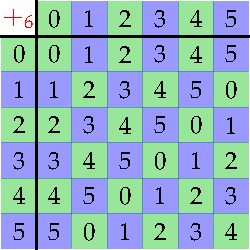
\includegraphics[scale=0.9]{factor-z6}\\
				Addition in $\Z_6$\\[5pt]
				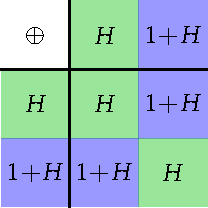
\includegraphics[scale=0.9]{factor-z6-2}\\
				Addition in $\{H,1+H\}$
			\end{tabular}
		\end{minipage}\smallbreak
		To save time, we verify all possibilities simultaneously. If $x\in a+H$ and $y\in b+H$, then
		\[
			(x+y)-(a+b)=(x-a)+(y-b)\in H\implies (x+y)+H=(a+b)+H
		\]
		Addition of cosets is therefore well-defined. The second table above suggests that the set of cosets forms a group under $\oplus$; indeed $\phi(x)=x+H$ defines an isomorphism of $\Z_2$ with this so-called \emph{factor group.}
	
		
% 	\exstart The set of (left) cosets for $H=\ip 4=\{0,4,8\}\le\Z_{12}$ is
% 	\[
% 		\bigl\{
% 			H,\ 1+H,\ 2+H,\ 3+H
% 		\bigr\}
% 		=\Bigl\{
% 			\{0,4,8\}, \{1,5,9\}, \{2,6,10\}, \{3,7,11\}
% 		\Bigr\}
% 	\]
% 	This feels like the cyclic group $\Z_4$ in disguise! To see this we need a binary operation: the natural approach is to use \textcolor{red}{addition} in $\Z_{12}$ to define addition of cosets via
% 	\[
% 		(a+H)\oplus(b+H):=(a\operatorname{\textcolor{red}{+}}b)+H
% 	\]
% 	This seems nice, though consider the computation more carefully:\vspace{-2pt}
% 	\begin{enumerate}\setcounter{enumi}{1}
% 	  \item[]\begin{enumeratea}
% 			\item \emph{\textbf{Choose} representatives} $a$ and $b$ in the respective cosets.
% 			\item \emph{Add within the original group} $a\operatorname{\textcolor{red}{+}}b\in\Z_{12}$.
% 			\item \emph{Take the left coset} $(a\operatorname{\textcolor{red}{+}}b)+H$.
% 		\end{enumeratea}
% 		If $\oplus$ is to make sense, the outcome $(a\operatorname{\textcolor{red}{+}}b)+H$ must be \emph{independent} of the \textbf{choices} in step (a). For instance, to properly conclude $(2+H)\oplus(3+H)=1+H$ we must check \emph{nine} possibilities
% 		\[
% 			a\in \{2,\textcolor{blue}{6},10\},\  b\in\{3,7,\textcolor{blue}{11}\} \implies a+b\in\{1,\textcolor{Green}{5},9\}
% 			\tag{one possibility is $\textcolor{blue}{6}+\textcolor{blue}{11}=\textcolor{Green}{5}\in\Z_{12}$}
% 		\]
% 		To save time, we verify all possibilities simultaneously. If $x\in a+H$ and $y\in b+H$, then
% 		\[
% 			(x+y)-(a+b)=(x-a)+(y-b)\in H\implies (x+y)+H=(a+b)+H
% 		\]
% 		Addition of cosets is therefore well-defined; indeed we'll shortly see that the set of (left) cosets forms a group under this natural addition. As you might guess, $\phi(x)=x+H$ defines an isomorphism of $\Z_4$ with this so-called \emph{factor group.}
		
	
		\item We repeat the process for the subgroup $H=\{e,\mu_1\}\le D_3$. The left cosets are
		\[
			H=\mu_1H=\{e,\mu_1\},\qquad
			\rho_1H=\mu_3H=\{\rho_1,\mu_3\},\qquad
			\rho_2H=\mu_2H=\{\rho_2,\mu_2\}
		\]
		As above, we attempt to define the `natural' operation on the set of left cosets
		\[
			aH\otimes bH:=(ab)H \tag{$ab$ is composition/multiplication within $D_3$}
		\]
		This time there is a serious problem, as the following two calculations show:
		\[
			\rho_1H\otimes\rho_1H =(\rho_1\rho_1)H =\rho_2H\qquad\qquad
			\mu_3H\otimes \mu_3H=(\mu_3\mu_3)H =eH =H
		\]
		This is a contradiction: since $\rho_1H=\mu_3H$, the results of both calculations \emph{should be the same}. The freedom of \textbf{choice} (part (a)) in the definition of $\otimes$ leads to different outcomes: the natural operation $\otimes$ \emph{does not exist} (and thus cannot produce a group structure!).
	\end{enumerate}
\end{examples*}



\boldsubsubsection{Well-definition of the Factor Group Structure}

The examples indicate that only some subgroups $H\le G$ behave nicely when trying to view the set of left cosets as a group. But which subgroups? To answer this question, we repeat some of our discussion abstractly. Let $H$ be a subgroup of $G$ and define the natural multiplication of left cosets\footnote{Since this operation arises naturally from that on $G$, we use the same notation (here multiplication).}
\[
	aH\cdot bH:=(ab)H \tag{$\ast$}
\]
This is well-defined precisely when
\[
	xH=aH,\ yH=bH \implies (xy)H=(ab)H \tag{$\dag$}
\]
If the natural multiplication of cosets is well-defined, the fact that $hH=H$ and $gH=gH$ for any $h\in H$, $g\in G$, tells us that
\[
 	(hg)H=gH,\text{ or equivalently }	g^{-1}hg\in H \tag{Theorem \ref{thm:cosetpart}}
\]
Since this holds \emph{for all} $g\in G$ and $h\in H$, Corollary \ref{cor:normalconj} says that \textbf{$\boldsymbol{H}$ is a normal subgroup of $\boldsymbol G$.} Not only is the converse also true, but the resulting structure forms a group under this operation.

\begin{thm}{}{}
	Suppose $H\le G$ and consider the natural operation ($\ast$) on the set of (left) cosets.
	\begin{enumerate}
	  \item ($\ast$) is well-defined if and only if $H$ is a normal subgroup of $G$.
	  \item	In such cases, $(\ast)$ defines a \emph{group structure} on the set of cosets.
	\end{enumerate}
\end{thm}

Since this process only works when $H$ is a normal subgroup, the prefix `left' is irrelevant.

\begin{defn}{}{}
	Given $H\triangleleft G$, the set of cosets is termed a \emph{factor group,} written $\quotient GH$ \ \ ('$G$ mod $H$').
\end{defn}

Factor group notation looks like division because if $G$ is finite, then $\nm{\quotient GH}=(G:H)=\frac{\nm G}{\nm H}$.

\begin{proof}
	\begin{enumerate}
	  \item\begin{description}
	  	\item[$(\Rightarrow)$] The above discussion shows that well-definition of $(\ast)$ implies $H\triangleleft G$.
	  	\item[$(\Leftarrow)$] Assume $H\triangleleft G$, and suppose $xH=aH$ and $yH=bH$. By Theorem \ref{thm:cosetpart}, $h:=x^{-1}a$ and $\tilde h:=y^{-1}b$ are both in $H$. But then,
		\[
			(xy)^{-1}(ab)=y^{-1}(x^{-1}a)b =y^{-1}hb =(y^{-1}hy)\tilde h
		\]
		which lies in $H$ by Corollary \ref{cor:normalconj} ($y^{-1}hy\in H$). We conclude that $(xy)H=(ab)H$ ($\dag$).
	  \end{description}
	  \item	Since the natural operation is well-defined, we need only verify the group axioms for $\left(\quotient GH,\cdot\right)$.
		\begin{description}
			\item[\normalfont\emph{Closure}:] Given $aH,bH\in\quotient GH$, we see that $aH\cdot bH=(ab)H$ is also coset.
			\item[\normalfont\emph{Associativity}:] $aH\cdot(bH\cdot cH)=aH\cdot(bc)H=a(bc)H$. Similarly $(aH\cdot bH)\cdot cH=(ab)cH$. By the associativity of $(G,\cdot)$, these cosets are identical.
			\item[\normalfont\emph{Identity}:] The \emph{identity coset} $H=eH$ does the job: $eH\cdot aH=(ea)H=aH=(ae)H=aH\cdot eH$.
			\item[\normalfont\emph{Inverse}:] $a^{-1}H\cdot aH=(a^{-1}a)H=eH=H$, etc., therefore $(aH)^{-1}=a^{-1}H$.\qedhere
		\end{description}
	\end{enumerate}
\end{proof}


\goodbreak


\boldsubsubsection{Factor Groups of $\Z$ (modular arithmetic done right)}

If $n$ is a positive integer, its integer multiples $n\Z=\ip n$ form a (normal) subgroup of $\Z$. The coset of $n\Z$ containing $x\in\Z$ is plainly
\[
	x+n\Z=\{x+kn:k\in\Z\}
	=\{y\in\Z:y\equiv x\negthickspace\negthickspace\pmod n\}
\]
This coset is precisely what we have been calling `$x$' in $\Z_n$! This provides the formal definition of $\Z_n$ (superseding Definition \ref{defn:znsimple}) and trivially demonstrating that $\Z_n$ is an abelian group.

\begin{defn}{}{}
	Let $n\in\N$. The group $\Z_n$ is the factor group $\quotient{\Z}{n\Z}$
\end{defn}

We typically drop the repeated $n\Z$ terms when calculating, recovering our familiar notation: e.g.
\[
	4+5=2\in\Z_7\quad\text{means}\quad (4+7\Z)+(5+7\Z)=2+7\Z \in\quotient{\Z}{7\Z}
\]


\boldsubsubsection{Factor Groups of Finite Cyclic Groups}

The first example on page \pageref{sec:factor} shows that $\quotient{\Z_6}{\ip 2} \cong\Z_2$. This generalizes in an obvious manner.

\begin{example}{}{}
	$\ip 5=\{0,5,10,15\}\le\Z_{20}$ has factor group
	\[
		\quotient{\Z_{20}}{\ip 5}=\bigl\{\ip 5,\ 1+\ip 5,\ 2+\ip 5,\ 3+\ip 5,\ 4+\ip 5\bigr\}
	\]
	which is isomorphic to $\Z_5$ via the isomorphism
	\[
		\psi:\Z_5\to\quotient{\Z_{20}}{\ip 5}:x\mapsto x+\ip 5
	\]
\end{example}


\begin{thm}{}{znisomdefn}
	If $d\mid n$, then $\quotient{\Z_n}{\ip d}\cong\Z_d$.
\end{thm}

If $s\nmid n$, Corollary \ref{cor:subscyclic} says that $\ip s=\ip d$ where $d=\gcd(s,n)$, whence $\quotient{\Z_n}{\ip s}\cong\Z_{\gcd(s,n)}$.

\begin{proof}
	Define $\psi:\Z_d\to\quotient{\Z_n}{\ip d}:x\mapsto x+\ip d$. We prove that this is an isomorphism.
	\begin{description}
		\item[\normalfont\emph{Well-definition/injectivity}:] For any $x,y\in\Z_d$,
		\begin{align*}
			x=y\ (\in\Z_d)&\iff x-y\in\ip d\iff x+\ip d=y+\ip d\\
			&\iff \psi(x)=\psi(y)
		\end{align*}
		\item[\normalfont\emph{Surjectivity}:] Any coset $x+\ip d$ (being $\psi(x)$) lies in $\operatorname{range}(\psi)$.	
		\item[\normalfont\emph{Homomorphism}:] For any $x,y\in\Z_d$,
		\begin{align*}
			\psi(x+y)&=(x+y)+\ip d =\bigl(x+\ip d\bigr)+\bigl(y+\ip d\bigr)\\
			&=\psi(x)+\psi(y) \tag*{\qedhere}		
		\end{align*}
	\end{description}
\end{proof}


\goodbreak


\boldsubsubsection{Finite Abelian Examples}

If $G$ is finite abelian, then any subgroup $H$ is normal and $\quotient GH$ is also a finite abelian group (exercise). By the Fundamental Theorem (\ref{thm:fund}), there are positive integers $m_1,\ldots,m_k$ for which
\[
	\quotient GH\cong \Z_{m_1}\times\cdots\times\Z_{m_k}
	\quad\text{and}\quad
	m_1\cdots m_k=\nm{\quotient GH}=(G:H)=\frac{\nm G}{\nm H}
\]
Our goal in these examples is to \emph{identify} $\smash{\quotient GH}$ as a direct product by finding suitable integers $m_k$.

\goodbreak

\begin{examples}{}{factorfiniteabelian}
	Let $G=\Z_4\times\Z_8$. We identify the factor group $\quotient GH$ for three subgroups $H$.
	\begin{enumerate}
	  \item Let $H=\ip{(0,1)}=\bigl\{(0,0),(0,1),\ldots,(0,7)\bigr\}$. The factor group $\quotient GH$ has order $\frac{\nm G}{\nm H}=\frac{4\cdot 8}8=4$, and is thus isomorphic either to $\Z_4$ or $\Z_2\times\Z_2$. Here are two naïve strategies for deciding which is correct; a third, more rigorous, approach will be discussed in Section \ref{sec:1stiso}.
	  \begin{description}
		  \item[Describe the cosets] Find a `nice' representative of each coset,
			\[
				(x,y)+H=(v,w)+H\iff (x,y)-(v,w)=(x-v,y-w)\in H\iff x=v
			\]
			Each coset contains a unique element $(x,0)$ where $x\in \Z_4$. We may therefore write
			\[
				\quotient{G}{H}=\Bigl\{H,\ (1,0)+H,\ (2,0)+H,\ (3,0)+H\Bigr\}
			\]
			\item[Orders of elements] Consider possible orders of cosets in $\quotient GH$,
			\[
				k\bigl((1,0)+H\bigr) =(k,0)+H=H\iff (k,0)\in H\iff 4\mid k \tag{$\ast$}
			\]
			Since $\quotient GH$ contains an element $(1,0)+H$ of order 4, it must be cyclic ($\cong \Z_4$).
		\end{description}
		Either approach essentially proves that $\psi:\Z_4\to\quotient GH:x\mapsto (x,0)+H$ is an isomorphism.
			
			 
	  \item Let $H=\ip{(0,2)}=\bigl\{(0,0),(0,2),(0,4),(0,6)\bigr\}$. This time $\nm{\quotient GH}=\frac{32}4=8$, so the factor group is isomorphic to one of $\Z_8$, $\Z_4\times\Z_2$ or $\Z_2\times\Z_2\times\Z_2$. We again follow our two strategies.
	  \begin{description}
		  \item[Describe the cosets]
			\[
				(x,y)+H=(v,w)+H\iff (x-v,y-w)\in H\iff 
				\begin{cases}
					\textcolor{red}{x=v},\text{ and}\\
					\textcolor{blue}{y-w\text{ is even}}
				\end{cases}
			\]
			from which the \emph{distinct} cosets may be written
			\[
				\quotient GH=\Bigl\{H,\ (1,0)+H,\ (2,0)+H,\ \ldots,\ (3,1)+H\Bigr\} =\Bigl\{(x,y)+H: \textcolor{red}{x\in\Z_4},\ \textcolor{blue}{y\in\Z_2}\Bigr\}
			\]
			In fact $\psi:\Z_4\times\Z_2\to\quotient GH:(x,y)\mapsto (x,y)+H$ is an isomorphism.
			\item[Orders of elements] Exactly as in ($\ast$), the coset $(1,0)+H$ has order 4. This rules out the possibility of $\Z_2\times\Z_2\times\Z_2$ (contains elements of maximum order 2).\par
	  	We rule out $\Z_8$ by observing that all elements of $\quotient GH$ have order dividing 4:
	  	\[
	  		4\bigl((x,y)+H\bigr)
	  		=(4x,4y)+H
	  		=(0,4y)+H
	  		=2y\bigl((0,2)+H\bigr)
	  		=H
	  	\]
			By process of elimination, we conclude that $\quotient GH\cong\Z_4\times\Z_2$.
	  \end{description}


		\goodbreak
	
	
		\item\label{ex:factoriso3} Let $H=\ip{(2,4)}=\bigl\{(0,0),(2,4)\bigr\}$. The factor group has order $\nm{\quotient GH}=\frac{32}2=16$ and we must consider \emph{five} non-isomorphic possibilities:\footnotemark{}
		\[
			\Z_{16},\quad \Z_2\times\Z_8,\quad \Z_4\times\Z_4,\quad \Z_2\times\Z_2\times\Z_4,\quad \Z_2\times\Z_2\times\Z_2\times\Z_2
		\]
	  \begin{description}
		  \item[Describe the cosets] This is a little trickier than before.
		  \begin{itemize}
	  		\item If $x=2n$ is even, then
	  		\[
	  			\textcolor{red}{(x,y)+H}
	  			=(2n,y)+H
	  			=n(2,4)+(0,y-4n)+H
	  			=(\textcolor{red}{0},y-4n)+H
	  		\]
	  		\item If $x=2n+1$ is odd, then
	  		\[
	  			\textcolor{red}{(x,y)+H}
	  			=(2n+1,y)+H
	  			=n(2,4)+(1,y-4n)+H
	  			=(\textcolor{red}{1},y-4n)+H
	  		\]
	  	\end{itemize}
	 		\textcolor{red}{Each coset} contains precisely one representative whose first entry is either \textcolor{red}{0} or \textcolor{red}{1}; we conclude that the distinct cosets of $H$ are represented by the sixteen elements
			\[
				(0,0),\ (0,1),\ \ldots,\ (0,7),\ (1,0),\ \ldots,\ (1,7) \tag{$(x,y)$ where $x\in\Z_2$, $y\in\Z_8$}
			\]
			This \emph{suggests} $\quotient GH\cong\Z_2\times\Z_8$, though our argument isn't quite a proof since the obvious `function' $\psi:\Z_2\times\Z_8\to\quotient GH:(x,y)\mapsto(x,y)+H$ isn't well-defined ($\psi(2,0)\neq\psi(0,0)$).
		  
			\item[Orders of Elements] The coset $(0,1)+H$ has order 8 in $\quotient GH$, since
			\[
				k\bigl((0,1)+H\bigr)=(0,k)+H=H\iff 8\mid k
			\]
			This reduces our options to $\Z_{16}$ and $\Z_2\times\Z_8$ since these are the only possibilities containing an element of order 8. Moreover, any coset has order dividing 8:
			\[
				8\Bigl((x,y)+H\Bigr)
				=(8x,8y)+H
				=(0,0)+H
			\]
	  	This rules out $\Z_{16}$, leaving $\Z_2\times\Z_8$ as the only possibility.
		\end{description}
	\end{enumerate}
\end{examples}


\footnotetext{%
	The previous examples might have created a false sense of security. While $H=\ip 2\times \ip 4$ is a direct product just like $G=\Z_4\times\Z_8$, we \emph{cannot divide groups} in the way you might expect:
	\[
		\quotient GH
		\mathrel{\textcolor{red}{\ncong}}
		\quotient{\Z_4}{\ip 2}\times\quotient{\Z_8}{\ip 4}
		\cong\Z_2\times\Z_2
	\]
	This \textcolor{red}{non-isomorphicity} is obvious since $\nm{\quotient GH}=16\neq 4=\nm{\Z_2\times\Z_2}$. See Exercise \ref{exs:normaldirectfactor} for why the first two examples seem to fit with such a `division' approach.  
}
		
	Strategy (b) might seem easier \& quicker right now, but it has its drawbacks: for instance, you cannot easily distinguish between (say) $\Z_4\times\Z_4$ and $\Z_2\times\Z_2\times\Z_4$ by considering orders of elements. Moreover, neither method suggests a suitable isomorphism: it can be checked (exercise) that
\[
	\psi:\Z_2\times\Z_8\to\quotient GH\to:(x,y)\mapsto (x,y-2x)+H
\]
does the job, though cooking up such a function requires some creativity! As we'll see in Section \ref{sec:1stiso}, a related approach offers a better way to tackle these problems\ldots 



\boldsubsubsection{Infinite or Non-Abelian Examples}

For factor groups of infinite or non-abelian groups, more varied strategies may be required.

\begin{examples}{}{normalmoreex}
	\exstart Given $W=\{(0,y):y\in\R\}\le \R^2$, each coset (vertical line) plainly contains a unique point $(x,0)$ on the $x$-axis. It is easily checked that $\psi:\R\to\quotient{\R^2}W:x\mapsto (x,0)+W$ is an isomorphism (this is a simplified version of Example \ref*{ex:cosetexs}.\ref{ex:cosetsubspace}).
	

	\begin{enumerate}\setcounter{enumi}{1}
	  \item Since $(D_n:R_n)=2$ ($n$ rotations and $n$ reflections!), we see that $\quotient{D_n}{R_n}$ has order 2 and is thus isomorphic to $\Z_2$. The function $\psi(0)=R_n$, $\psi(1)=\{\text{reflections}\}$ is an isomorphism. Note how the factor group calculation $(\mu_iR_n)(\mu_jR_n)=R_n$ ($\leftrightsquigarrow 1+1=0\in\Z_2$) says that the composition of two reflections is a rotation.
	  
	  \item $\ip{2\pi}=2\pi\Z=\{2\pi n:n\in\Z\}$ is a subgroup of $(\R,+)$. In any given coset, there is a unique real number $x$ such that $0\le x<2\pi$ (think `take the remainder modulo $2\pi$'). It follows that
	  \[
	  	\quotient{\R}{2\pi\Z}=\bigl\{x+2\pi\Z:x\in[0,2\pi)\bigr\}
	  \]
	  Moreover, the function
	  \[
	  	\mu:\quotient\R{2\pi\Z}\to S^1:x+2\pi\Z\mapsto e^{ix}
	  \]
	  is a well-defined isomorphism. The factor group construction can be visualized as wrapping the real line infinitely many times around a circle of radius 1 (circumference $2\pi$).
	  
	  \item\label{ex:a4normal} By Exercise \ref*{sec:cosetnormal}.\ref{exs:va4}, the Klein four-group identified as $V=\bigl\{
				e,(1\,2)(3\,4),(1\,3)(2\,4),(1\,4)(2\,3)
			\bigr\}$
% 	  \[
% 			V=\bigl\{
% 				e,(1\,2)(3\,4),(1\,3)(2\,4),(1\,4)(2\,3)
% 			\bigr\}
% 		\]
	  is a normal subgroup of the alternating group $A_4$. The factor group has order $(A_4:V)=\frac{12}4=3$, whence $\quotient{A_4}{V}\cong\Z_3$: can you find an explicit isomorphism?\par
	  It is harder to check, but we'll see later (Section \ref{sec:conj}) that $\quotient{S_4}{V}\cong S_3$.
	  
	  
	  \item Consider $H=\ip{(2,1)}\le\Z\times\Z_4=G$. Since $G$ and $H$ are infinite, we cannot count cosets using the index formula. Instead we find a representative of each coset similarly to Example \ref*{ex:factorfiniteabelian}.\ref{ex:factoriso3}.
	  \[
	  	(x,y)+H=
	  	\begin{cases}
	  		(2n,y)+H=(0,y-n)+H&\text{if $x=2n$ is even}\\
	  		(2n+1,y)+H=(1,y-n)+H&\text{if $x=2n+1$ is odd}
	  	\end{cases}
	  \]
	  There is a \emph{unique representative} in each coset either of the form $(0,z)$ or $(1,z)$, where $z\in\Z_4$. We conclude that there are $2\cdot 4=8$ cosets. Since the factor group is abelian (Exercise \ref{exs:gmodhabelian}), it must be isomorphic to one of $\Z_8$, $\Z_2\times\Z_4$ or $\Z_2\times\Z_2\times\Z_2$. To identify which, compute
	  \[
	  	4\bigl((x,y)+H\bigr)=(4x,4y)+H=(0,-2x)+H=H \iff 2\mid x
	  \]
	  Since $(1,0)+H$ has order 8, the factor group is cyclic and we have an explicit isomorphism
	  \[
	  	\psi:\Z_8\to\quotient GH:x\mapsto (x,0)+H
	  \]
	  
	  \item\label{ex:hardgmodh} Let $H=\ip{(1,2)}\le\Z\times\Z=G$. We play a similar trick to before
	  \[
	  	(x,y)+H =(0,y-2x)+(x,2x)+H =(0,y-2x)+H
	  \]
	  It follows that there is a unique representative of the form $(0,z)$ in each coset and we suspect $\quotient GH\cong\Z$. Indeed it can be verified that $\psi\bigl((x,y)+H\bigr)=y-2x$ is an isomorphism. 
	
		% 	\item\label{ex:nastyiso} Consider $H=\ip{(1,2,2)}\le G=\Z_5\times\Z_6\times\Z$. Since $G$ is infinite, we cannot simply apply the index formula to count cosets. Instead we appeal to the division algorithm.\smallbreak
		
		% 	Given $(x,y,z)$, we may subtract as many multiples of $(1,2,2)$ as we like while remaining in the same coset. It follows that each coset $(x,y,z)+H$ has a unique representative with $z=0$ or 1. In essence we are writing $z=2q+r$ where $r=0,1$ and observing that
		%   \[(x,y,z)+H=(x-q,y-2q,r)+H\]
		%   Since we have a free choice of $x\in\Z_5$ and $y\in\Z_6$ we see that there are precisely $5\cdot 6\cdot 2=60$ cosets. Since the factor group is abelian of order $60$, it must be isomorphic to one of two groups
		%   \[\Z_{60}\cong \Z_{2^2}\cdot\Z_3\times\Z_5\qquad \Z_2\times\Z_{30}\cong\Z_2\times\Z_2\times\Z_3\times\Z_5\]
		%   We distinguish between these by considering the possible orders of elements: the former requires an element of order 60. However,
		%   \[30\bigl((x,y,z)+H\bigr)=(30x,30y,30z)+H=(30x-15z,30y-30z,0)+H=H\]
		%   whence every element of the factor group $\quotient GH$ has order dividing 30.\par
		%   By elimination, we conclude that $\quotient GH\cong \Z_2\times\Z_{30}$.%\\
		%   An alternative approach, requiring a little creativity, involves spotting that
		%   \[\phi:\Z_5\times\Z_6\times\Z\mapsto\Z_5\times\Z_6\times\Z_2:(x,y,z)\mapsto (2x-z\spmod 5,y-z\spmod 6,z\spmod 2)\]
		%   is a surjective homomorphism with $\ker\phi=H$. The 1st isomorphism theorem then says that
		%   \[\mu:\quotient GH\cong \Z_5\times\Z_6\times\Z_2:(x,y,z)+H\mapsto (2x-z\spmod 5,y-z\spmod 6,z\spmod 2)\]
		
	\end{enumerate}
\end{examples}


\clearpage


\begin{exercises}
	Key concepts:
	\begin{quote}
		\emph{Factor group\qquad $\quotient GH$ a group $\iff H\triangleleft G$\qquad $\Z_n:=\quotient{\Z}{n\Z}$\qquad identifying $\quotient GH$}
	\end{quote}
	
	\begin{enumerate}
	  \item List the cosets of the subgroup $H=\ip{3}$ in $G=\Z_{15}$. By mimicking the proof of Theorem \ref{thm:znisomdefn}, show that $\psi:\Z_3\mapsto \quotient GH:x\mapsto x+H$ is a well-defined homomorphism.
% 	  \[
% 	  	\psi:\Z_3\mapsto \quotient GH:x\mapsto x+H
% 	  \]
	
		
		\item  (Recall Exercise \ref*{sec:cosetnormal}.\ref{exs:VfactorV})\lstsp If $H=\bigl\{(0,0),(0,2),(2,0),(2,2)\bigr\}$, identify the factor group $\quotient{\Z_4\times\Z_4}H$.
		
		
		\item Identify the factor group $\quotient GH$ where $H=\ip{(2,4)}\le G=\Z_4\times\Z_6$.
		  %\item Repeat with the subgroup $H=\ip 2\times\ip 4$ (\emph{this is a trick question!})
		
		
		\item\begin{enumerate}
		  \item Let $G=\Z_9\times\Z_9$ and $H=\ip{(3,6)}$. Identify $\quotient GH$ by showing that every element of the factor group has order at most 9 and that it contains an element of order 9.
		  
		  \item Repeat with $H=\ip 3\times\ip 6$ \ (\emph{this \textbf{isn't} a trick question}).
		\end{enumerate}
	  
	  
		\item Let $G$ be any group. To what groups are $\quotient G{\{e\}}$ and $\quotient GG$ isomorphic?
		
	
		\item\label{exs:gmodhabelian}\begin{enumerate}
		  \item If $G$ is abelian and $H\le G$, prove that $\quotient GH$ is abelian.
		  
		  \item If $\quotient GH$ is abelian, can we conclude that $G$ and/or $H$ is abelian? Explain.
		\end{enumerate}
		
	
	 	\item (See Examples \ref{ex:factorfiniteabelian})\lstsp Let $G=\Z_4\times\Z_8$. Prove that each $\psi$ is a well-defined homomorphism:
		\begin{enumerate}\itemsep0pt
			\item $H=\ip{(0,1)}$, \ $\psi:\Z_4\to\quotient GH:x\mapsto (x,0)+H$
			\item $H=\ip{(0,2)}$, \ $\psi:\Z_4\times\Z_2\to\quotient GH:(x,y)\mapsto (x,y)+H$
			\item $H=\ip{(2,4)}$, \ $\psi:\Z_2\times\Z_8\to\quotient GH:(x,y)\mapsto (x,y-2x)+H$
		\end{enumerate}
		(\emph{Bijectivity follows from the description of the cosets, though proving injectivity might be instructive.})
		
		
		\item Revisit Exercise \ref*{sec:lagrange}.\ref{exs:zsqrt2subgroup}. The factor group $\quotient GH$ is abelian and of order 6, whence it is cyclic. Prove this explicitly by finding a generator and thus an isomorphism $\psi:\Z_6\to\quotient GH$.
		
		
		\item\begin{enumerate}
	  	\item Let $G$ be a cyclic group with subgroup $H$. Prove that $\quotient GH$ is cyclic.
	  	\item If $\quotient GH$ is cyclic, does it follow that $G$ is cyclic? Explain.
		\end{enumerate}
	
	
		\item In Example \ref*{ex:normalmoreex}.\ref{ex:a4normal} we saw that $\Z_3\cong\quotient{A_4}{V}$. Find an explicit isomorphism.
			
	
		\item Exercise \ref*{sec:cosetnormal}.\ref{exs:d4normal} showed that $\{\rho_0,\rho_2\}$ is a normal subgroup of $D_4$. To what well-known group is the factor group $\quotient{D_4}{\{\rho_0,\rho_2\}}$ isomorphic? Prove your assertion.
		
	
		\item\begin{enumerate}
		  \item Identify the factor group $\quotient{S_n}{A_n}\cong K$ where $K$ is some well-understood basic group. Describe an explicit isomorphism $\psi:K\to\quotient{S_n}{A_n}$ and verify that it is such.
		  \item Repeat for the factor group $\quotient{\rO_n(\R)}{\rSO_n(\R)}$.
		\end{enumerate}
		
		
		\item\label{exs:normaldirectfactor} (Recall Exercise \ref*{sec:cosetnormal}.\ref{exs:directprodfactor})\lstsp Suppose $G=H\times K$, $J\triangleleft H$ and $\widehat J=J\times\{e_K\}$. Prove that $\quotient G{\widetilde J}=\quotient HJ\times K$.\par
		Can you quickly verify Examples \ref{ex:factorfiniteabelian}.1, 2, and \ref{ex:normalmoreex}.1 in this language?
		
		
		\item Let $H=\ip{(2,3)}\le G=\Z_5\times \Z$. Prove that $\quotient GH\cong \Z_{15}$.
		
		
		\item Verify the claim in Example \ref*{ex:normalmoreex}.\ref{ex:hardgmodh} that $\psi\bigl((x,y)+H\bigr)=y-2x$ is an isomorphism.
		
		
		\item (Hard!)\lstsp Let $G=\Z_{10}\times\Z_6\times\Z$ and $H=\ip{(4,2,3)}$. Identify $\quotient GH$ as a direct product $\Z_m\times\Z_n$.\par
		(\emph{Hint: show that exactly one representative of the coset $(x,y,z)+H$ has $z$ either 0, 1 or 2})
		
		
		%   \item Let $G=\Z_{10}\times\Z_6\times\Z$ and $H=\ip{(4,2,3)}$. Since the groups are infinite, we cannot use the index formula to count cosets.
	%   We sketch the process for identifying $\quotient GH$: the details of parts (b), (c) and (d) are an exercise with some hints.
	%   \begin{enumerate}
	%     \item Apply the division algorithm: $z=3q+r$ where $r=0,1,2$ and observe that
	%   	\[(x,y,z)+H=(x,y,z)-q(4,2,3)+H=(x-4q,y-2q,r)+H\]
	%   	Every coset therefore contains precisely one element $(x,y,z)$ where either $z=0,1$ or 2.
	%   	\item The elements $(x,y,0),(x,y,1)$ and $(x,y,2)$ where $x\in\Z_{10}$ and $y\in\Z_6$ are shown to lie in different cosets. There are therefore $180=2^2\cdot 3^2\cdot 5$ cosets which yield four non-isomorphic possibilities for the factor group:
	%   	\[\Z_{180},\ \ \Z_2\times\Z_{90},\ \ \Z_3\times\Z_{60},\ \ \Z_6\times\Z_{30}\]
	%   	\item The coset $(1,1,1)+H$ has order 90.
	% %   	\[n(1,1,1)\in H\implies n=3k\implies (n-2k,n-4k,0)\in H\]
	% %   	\begin{align*}
	% %   		3k(1,1,1)+H&=(3k,3k,3k)+H=(3k,3k,3k)-k(4,2,3)+H\tag*{(since $(4,2,3)\in H$)}\\
	% %   		&=(-k,k,0)+H\\
	% %   		&=H\iff 10\mid k\ \text{and}\ 6\mid k \iff 30\mid k\iff 90\mid n
	% %   	\end{align*}
	%   	\item Every coset $(x,y,z)+H$ has order dividing 90.
	%   \end{enumerate}
	%   We conclude that $\quotient GH\cong \Z_2\times\Z_{90}$.
	
	% 	\begin{itemize}
	%   \item : if two such were in the same coset, then
	%   \begin{align*}
	%   (x_1,y_1,0)-(x_2,y_2,0)\in H&\iff (x_1-x_2,y_1-y_2,0)\in H\\
	%   &\iff\begin{cases}
	%   x_1\equiv x_2\pmod{10}\\
	%   \qquad\quad\text{and}\\
	%   y_1\equiv y_2\pmod{6}
	%   \end{cases}
	%   \end{align*}
	%   Similarly all the elements $(x,y,1)$ and $(x,y,2)$ lie in different cosets.
	%   \item It follows that the elements $(x,y,0)$, $(x,y,1)$ and $(x,y,2)$ are representatives of different cosets, and that all cosets have one such representative. There are therefore $10\cdot 6\cdot 3=180$ distinct cosets whence the factor group $\quotient GH$ is abelian of order 180.
	%   \item The prime decomposition of $180$ is $2^2\cdot 3^2\cdot 5$: there are, up to isomorphism, \emph{four} abelian groups of order 180, namely
	%   \begin{gather*}
	%   \Z_4\times\Z_9\times\Z_5\cong\Z_{180}\\
	%   \Z_2\times\Z_2\times\Z_9\times\Z_5\cong\Z_2\times\Z_{90}\\
	%   \Z_4\times\Z_3\times\Z_3\times\Z_5\cong\Z_3\times\Z_{60}\\
	%   \Z_2\times\Z_2\times\Z_3\times\Z_3\times\Z_5\cong\Z_6\times\Z_{30}
	%   \end{gather*}
	%   How do we distinguish between these? As before, we look for elements of a particular order (lots of scratch work may be required in general!).
	%   \item Compute the order of the coset $(1,1,1)+H$. Certainly its order must be divisible by 3, since the third entry of
	%   \[n(1,1,1)=(n,n,n)\in H\]
	%   requires $3\mid n$. Thus let $n=3k$. Now
	%   \begin{align*}
	%   3k(1,1,1)+H&=(3k,3k,3k)+H=(3k,3k,3k)-k(4,2,3)+H\tag*{(since $(4,2,3)\in H$)}\\
	%   &=(-k,k,0)+H\\
	%   &=H\iff 10\mid k\ \text{and}\ 6\mid k \iff 30\mid k\iff 90\mid n
	%   \end{align*}
	%   Since $\quotient GH$ contains an element of order 90, our choices are narrowed to $\Z_{180}$ and $\Z_2\times\Z_{90}$.
	%   \item We show that \emph{every} element of $\quotient GH$ has order dividing 90:
	%   \begin{align*}
	%   90\bigl((x,y,z)+H\bigr)&=(90x,90y,90z)-30z(4,2,3)+H=(90x-120z,90y-60z,0)+H\\
	%   &=(0,0,0)+H
	%   \end{align*}
	%   We conclude that $\quotient GH\cong\Z_2\times\Z_{90}$. Phew!
	% \end{itemize}
	% You can check (it's hard!) that the function
	% \[\psi:\Z_2\times\Z_{90}\to\quotient{(\Z_{10}\times\Z_6\times\Z)}{\ip{(4,2,3)}}:(x,y)\mapsto(y,3x+y,y)+H\]
	% is an isomorphism, though you'd have to be truly inspired to conjecture this out of thin air!
		
		
	\end{enumerate}

\end{exercises}






\subsection{The First Isomorphism Theorem}\label{sec:1stiso}

We've seen that all kernels of group homomorphisms are normal subgroups. In fact \emph{all} normal subgroups are the kernel of some homomorphism.

\begin{thm}{Canonical Homomorphism}{}
	Let $G$ be a group and $H\triangleleft G$. Then the function
	\[
		\gamma:G\to \quotient GH
		\quad\text{defined by}\quad 
		\gamma(g)=gH
	\]
	is a homomorphism with $\ker\gamma=H$.
\end{thm}

\begin{proof}
	Since $H$ is normal, $\quotient GH$ is a group. By the definition of multiplication in $\quotient GH$,
	\[
		\gamma(g_1)\gamma(g_2)
		=g_1H\cdot g_2H
		=(g_1g_2)H
		=\gamma(g_1g_2)
	\]
	whence $\gamma$ is a group homomorphism. Moreover, the identity in the factor group is $H$, whence
	\[
		\ker\gamma=\{g\in G:\gamma(g)=H\} 
		=\{g\in G:gH=H\}=H
		\tag*{\qedhere}
	\]
\end{proof}

This might feel a little sneaky and unsatisfying; we'd perhaps have preferred a homomorphism that doesn't have a factor group as its image! However, a companion result says that, among all homomorphisms with the same kernel, $\gamma$'s appearance is unavoidable.

\begin{thm}{1\st{} Isomorphism Thm}{}
	Let $\phi:G\to L$ be a homomorphism with kernel $H$. Then
	\[
		\mu:\quotient GH\to\image\phi
		\quad \text{defined by}\quad 
		\mu(gH)=\phi(g)
	\]
	is an isomorphism. Otherwise said, $\quotient G{\ker\phi}\cong\image\phi$.
\end{thm}


\begin{minipage}[t]{0.69\linewidth}\vspace{-5pt}
	These results may be summarized in a \emph{commutative diagram:} a homomorphism $\phi:G\to L$ \emph{factors} as $\phi=\mu\circ\gamma$, where $\gamma$ is the canonical homomorphism with kernel $\ker\phi$. This theorem is very important, and has analogues in several other parts of mathematics: e.g., the rank--nullity theorem from linear algebra is of close kin.
\end{minipage}
\hfill
\begin{minipage}[t]{0.3\linewidth}\vspace{-5pt}
	\flushright$\xymatrix{%
		G \ar[rr]^{\phi} \ar[dr]_\gamma && \image\phi\\
		& \quotient G{\ker\phi} \ar[ur]_{\mu} &
	}$
\end{minipage}



\begin{proof}
	The factor group exists since $\ker\phi\triangleleft G$ (Lemma \ref{lemm:homosub}). We check the isomorphism properties:
  \begin{description}
		\item[\normalfont\emph{Well-definition and Bijectivity}:] These are immediate from Lemma \ref{lemm:homobij} after writing $H=\ker\phi$:
		\[
			g_1H=g_2H
			\iff \phi(g_1)=\phi(g_2)
			\iff \mu(g_1H)=\mu(g_2H)
		\]
		\item[\normalfont\emph{Homomorphism}:] For all $g_1H,g_2H\in\quotient GH$,
		\begin{align*}
			\mu(g_1H\cdot g_2H)
			&=\mu(g_1g_2H)=\phi(g_1g_2)
				\tag{definition of $\mu$}\\ 
				&=\phi(g_1)\phi(g_2)
				\tag{$\phi$ is a homomorphism}\\
			&=\mu(g_1H)\mu(g_2H)
		\end{align*}
  \end{description}
	We conclude that $\mu$ is an isomorphism.
\end{proof}


\begin{examples}{}{}
	\exstart Let $\phi:\Z_{12}\to\Z_{20}$ be the homomorphism $\phi(x)=5x\!\!\pmod{20}$ (Example \ref{ex:homoz12-20}). Its kernel and image are
	\begin{gather*}
		\ker\phi
		=\bigl\{x\in\Z_{12}:5x\equiv 0\negthickspace\pmod{20}\bigr\}
		=\{0,4,8\}
		=\ip 4\le \Z_{12}\\
		\image\phi=\{5x\in\Z_{20}:x\in\Z_{12}\}
		=\{0,5,10,15\}
		=\ip{5}\le\Z_{20}
	\end{gather*}
	The relevant factor group is
	\begin{align*}
		\quotient{\Z_{12}}{\ker\phi}
		&=\Bigl\{\{0,4,8\},\{1,5,9\},\{2,6,10\},\{3,7,11\}\Bigr\}
		=\bigl\{\ip 4,1+\ip 4,2+\ip 4,3+\ip 4\bigr\}
	\end{align*}
	The canonical homomorphism $\gamma$ and the isomorphism $\mu$ are\vspace{-5pt}
	\begin{enumerate}\setcounter{enumi}{1}
	  \item[]\begin{quote}
			$\SelectTips{cm}{}\xymatrix @C40pt @R0pt{%
				\rlap{$\gamma(x)=x+\ip 4$} &&& \Z_{12} \ar@{->}[r]_-{\textstyle\gamma} \ar@{->}@/^15pt/[rr]^{\textstyle\phi} & \quotient{\Z_{12}}{\ip 4} \ar@{->}[r]_-{\textstyle\mu} & \image\phi\\
				\rlap{$\mu\bigl(x+\ip 4\bigr)=5x$} &&& x \ar@{|->}[r] & x+\ip 4 \ar@{|->}[r] & 5x
			}$
		\end{quote}
	  
	\item (Example \ref{ex:normalmoreex}.1)\lstsp $\phi:\R\to(\C^\times,\cdot):x\mapsto e^{ix}$ is a homomorphism with
  \[
  	\ker\phi=\{x\in\R:e^{ix}=1\}=\ip{2\pi}=2\pi\Z\le\R
  	\quad\text{and}\quad 
  	\image\phi=S^1
  	\tag{$S^1$ is the circle group}
  \]
  The canonical homomorphism $\gamma$ and the isomorphism $\mu$ from the theorem are
  \[
  	\gamma:\R\to\quotient{\R}{\ip{2\pi}}:x\mapsto x+\ip{2\pi}
  	\quad\text{and}\quad
  	\mu:\quotient\R{\ip{2\pi}}\to S^1:x+\ip{2\pi}\mapsto e^{ix}
  \]
  Note that $\mu$ is precisely the isomorphism we saw previously!
  
  \item $\phi:\Z\times\Z\to\Z:(x,y)\mapsto 3x-2y$ is a homomorphism. Moreover
  \[
  	\phi(x,y)=(0,0)\iff 3x=2y\iff (x,y)=(2n,3n)\text{ for some $n\in\Z$}
  \]
  We conclude that $\ker\phi=\ip{(2,3)}$. The canonical homomorphism is
  \[
  	\gamma:\Z\times\Z\to
  	\quotient{\Z\times\Z}{\ip{(2,3)}}:
  	(x,y)\mapsto (x,y)+\ip{(2,3)}
  \]
  Since $\phi$ is surjective (e.g., $n=\phi(n,n)$), the 1\st{} isomorphism theorem tells us that
  \[
  	\quotient{\Z\times\Z}{\ip{(2,3)}}\cong\Z
  	\quad\text{via}\quad 
  	\mu\bigl((x,y)+\ip{(2,3)}\bigr)=3x-2y
  \]
  
  \item $\phi(x,y)=(x,y-x)$ is a well-defined homomorphism $\phi:\Z\times\Z_6\to\Z_3\times\Z_6$. Moreover,
  \begin{gather*}
  	\phi(x,y)=(0,0)\iff
  	\begin{cases}
  		x=3k,\text{ and}\\
  		y=x=3k\in\Z_6
  	\end{cases}\\
  	\text{whence}\quad
  	\ker\phi=\ip{(3,3)}=\bigl\{\ldots,(-6,0),(-3,3),(0,0),(3,3),(6,0),\ldots\bigr\}
  \end{gather*}
  Plainly $\phi$ is surjective ($(m,n)=\phi(m,n+m)$); we conclude that $\quotient{\Z\times\Z_6}{\ip{(3,3)}}\cong\Z_3\times\Z_6$ via the isomorphism $\mu\bigl((x,y)+\ip{(3,3)})=(x,y-x)$.
	\end{enumerate}
\end{examples}

\vfil

\goodbreak


With a little creativity, the 1\st{} isomorphism theorem may be applied to the identification of factor groups: given $H\triangleleft G$, cook up a homomorphism $\phi:G\to L$ with $\ker\phi=H$, then $\quotient GH\cong\image\phi$. We revisit some examples from the previous section in this context.

\begin{examples*}{\ref{ex:factorfiniteabelian},\,mk.II}{}
	Let $G=\Z_4\times\Z_8$. For each subgroup $H$, we describe a homomorphism $\phi:G\to L$ with $\ker\phi =H$. While there are often several possible choices for $\phi$, ours will line up with what we saw in the original incarnations. Hopefully you'll feel that the reasons for our choices are independent of earlier discussions. %Note that if $\phi(1,0)=(a,c)$ and $\phi(0,1)=(b,d)$, then
	%\[\phi(x,y)=(ax+by,cx+dy)\]
	\begin{enumerate}
	  \item Given $H=\ip{(0,1)}$, we need a homomorphism where $\phi(0,1)$ is the identity. A simple way to do this is to ignore $y$ and define
	  \[
	  	\phi:\Z_4\times\Z_8\to\Z_4:(x,y)\mapsto x
	  \]
	  This indeed has kernel $\ker\phi=\{(0,y):y\in\Z_8\} =H$, whence
	  \[
	  	\quotient GH\cong\image\phi=\Z_4
	  \]
	  via the isomorphism $\mu:(x,y)+H\mapsto x$.\par
	  To connect back to the original problem, note that $(x,y)+H=(x,0)+H$ for all $x,y$, whence $\mu$ is the \emph{inverse} of the isomorphism $\psi:x\mapsto (x,0)+H$ stated previously!
	
	  \item Given $H=\ip{(0,2)}$ we require $\phi(0,2)$ to be the identity. This may be achieved by taking $y$ modulo 2 and defining
	  \[
	  	\phi:\Z_4\times\Z_8\to\Z_4\times\Z_2:(x,y)\mapsto (x,y)
	  \]
	  This is a well-defined ($\textcolor{red}{\phi(x+4m,y+8n)=\phi(x,y)}$, since $2\mid 8$) homomorphism with the required kernel $=H$. Moreover, $\phi$ is surjective, whence
	  \[
	  	\quotient GH\cong \image\phi= \Z_4\times\Z_2
	  \]
	  via the isomorphism $\mu\bigl((x,y)+H\bigr) =(x,y)$. Once again $\mu$ is the inverse of $\psi(x,y)=(x,y)+H$ in the original example.
	  
	  \item For the last version, finding a homomorphism with kernel $H=\ip{(2,4)}=\{(0,0),(2,4)\}$, is somewhat trickier. One approach is to observe that
	  \[
	  	(x,y)\in H\iff x\equiv 0\negthickspace\pmod 2\ \text{ and }\ y-2x\equiv 0\negthickspace\pmod 8
	  \]
	  We therefore choose
	  \[
	 		\phi:\Z_4\times\Z_8\to\Z_2\times\Z_8:(x,y)\mapsto\bigl(x,y-2x\bigr)
	 	\]
	  It is worth checking that this is \textcolor{red}{well-defined}: the $\textcolor{red}{2}x$ in the second factor is crucial! Certainly $\phi$ has the correct kernel. It is moreover surjective, e.g.\ $(m,n)=\phi(m,n+2m)$, whence
	  \[
	  	\quotient GH\cong\image\phi=\Z_2\times\Z_8
	  \]
	  via the isomorphism $\mu\bigl((x,y)+H\bigr)=(x,y-2x)$.
	\end{enumerate}
\end{examples*}


\goodbreak

\begin{exercises}{}{}
	Key concepts:
	\begin{quote}
		\emph{Canonical homomorphism $\gamma:G\to\quotient GH$\qquad 1\st{} isomorphism theorem $\mu:\quotient G{\ker\phi}\cong\image\phi$}
	\end{quote}
	
	\begin{enumerate}
	  \item Let $\phi:\Z_{18}\to\Z_{12}$ be the homomorphism $\phi(x)=10x$. 
	  \begin{enumerate}
	    \item Find the kernel of and image of $\phi$.
	    \item List the elements of the factor group $\smash[b]{\quotient{\Z_{18}}{\ker\phi}}$.
	    \item State an explicit isomorphism $\mu:\quotient{\Z_{18}}{\ker\phi}\to\image\phi$.
	    \item To what basic group $\Z_n$ is the factor group isomorphic?
	  \end{enumerate}
	  
	 	
	 	\item Repeat the previous question for the homomorphism $\phi:\Z\to\Z_{20}:x\mapsto 8x$.
	  
	  
	  \item For each function $\phi:\Z\times\Z\to\Z$, find the kernel and identify the factor group $\smash{\quotient{\Z\times\Z}{\ker\phi}}$.
	  \begin{enumerate}
	    \item $\phi(x,y)=3x+y$\qquad\qquad (b)\lstsp $\phi(x,y)=2x-4y$
	  \end{enumerate}  
	  
	    
	  \item\begin{enumerate}
	  	\item If a subgroup $H$ of $G=\Z_{15}\times\Z_3$ has order 5, find its elements.
			\item Show that $\phi(x,y)=(x,y)$ is a homomorphism $\phi:G\to\Z_3\times\Z_3$ with $\ker\phi=H$.
			\item What does the 1\st{} isomorphism theorem tell us about the factor group $\quotient GH$?
		\end{enumerate}
	  
	  
	  \item Suppose $G$ is a finite group with normal subgroup $H$ and that $\phi:G\to L$ is a homomorphism with $\ker\phi=H$. Prove that $(G:H)\le \nm L$ with equality if and only if $\phi$ is surjective.
	  
	  
	  \item Consider the map $\phi:\Z\times\Z_{12}\to \Z_3\times\Z_6$ defined by
	  \[
	  	\phi(x,y)=\bigl(2x+y,y\bigr)
	  \]
	  \begin{enumerate}
	    \item Verify that $\phi$ is a well-defined homomorphism.
	    \item Compute $\ker\phi$ and identify the factor group $\quotient{\Z\times\Z_{12}}{\ker\phi}$
	  \end{enumerate}
	  
	  
	  \item Let $H=\ip{(3,1)}\le G=\Z_9\times\Z_3$. Find an explicit homomorphism $\phi:G\to\Z_9$ whose kernel is $H$, and thus identify the factor group $\quotient GH$.\par
	  (\emph{Hint: $(x,y)\in H=\{(0,0),(3,1),(6,2)\}\iff\ldots$})
	  
	  \item Consider $H=\ip{(3,3)}\le G=\Z_9\times\Z_9$. Find a surjective homomorphism $\phi:G\to\Z_3\times\Z_9$ whose kernel is $H$ and hence prove that $\quotient GH\cong\Z_3\times\Z_9$.
	  
	  
	  \item Let $\phi:S^1\to S^1:z\mapsto z^2$.
	  \begin{enumerate}
	    \item Find the kernel of $\phi$ and describe the canonical homomorphism $\gamma:S_1\to\smash{\quotient{S^1}{\ker\phi}}$.
	    \item What does the first isomorphism theorem say about the factor group $\smash{\quotient{S^1}{\ker\phi}}$.
	    \item For each $n$, identify the factor group $\smash{\quotient{S^1}{U_n}}$, where $U_n$ is the group of $n\th$ roots of unity.
	  \end{enumerate}
	 
	  %\item Recall Example \ref*{ex:normalmoreex}.\ref{ex:nastyiso}. If $H=\ip{(1,2,2)}\le G=\Z_5\times\Z_6\times\Z$, try to find a surjective homomorphism $\phi:G\to \Z_5\times\Z_6\times\Z_2$ with $\ker\phi=H$.
	\end{enumerate}
\end{exercises}

